\chapter{Анализ литературы, патентов и обзор практики рецикла урана}\label{ch:ch1}

\section{Теоретические основы}


\subsection{Основы теории разделения в каскадах}
\textcolor{red}{Базовые понятия (разделительный элемент, симметричн.-противоточное соединений, каскад) + основные уравнения (балансы, срез, коэффициенты разделения ступеней)}
\dots

\subsection{Модельные каскады}


Вычислительные эксперименты, проводимые с целью исследования каскадов, опираются на использование специальных математических моделей, которые будут представлены в текущем разделе. Они позволяют заметно упростить изучение закономерностей изотопно-селективного массопереноса в разделительных каскадах. Этот вспомогательный инструмент принято называть модельным каскадом.

Физико-математические модели каскадов основанны на фундаментальных законах, таких как закон сохранения вещества. Эти теоретические описания адекватны процессу разделения в реальных разделительных аппаратах, в качестве которых сегодня, как правило, используются газовые центрифуги.

В области математического моделирования разделительных каскадов на сегодня разработан обширный набор расчетных моделей, которые могут быть применены в том числе и к задаче обогащения регенерированного урана. В нашем случае для разделения изотопов урановой смеси может быть применен ряд специальных теоретических моделей.

Наиболее общая из таких моделей называется «квазиидеальным» каскадом, где предполагается постоянство коэффициентов деления (срезов) потоков ($\theta$ делит входной поток на $\theta$ и $1 - \theta$ соответственно) по каскадным ступеням \cite{yamamotoMulticomponentIsotopeSeparating1978}. В настоящее время он используется в двух приближениях: со слабым обогащением (Q-каскад \cite{borisevichNewApproachOptimize2011, kolokoltsovDesignCascadesSeparating1970, zengQCascadeExplanation2012}) и произвольным обогащением (квазиидеальный каскад \cite{sulaberidzeSpecialFeaturesEnrichment2006}). Обе математические модели предлагают выбор профиля потока в каскаде, следовательно, дают возможность добиться наиболее эффективного обогащения целевого компонента. Такой подход значительно упрощает как анализ закономерностей массообмена в каскаде для многокомпонентного разделения, так и соответствующий расчет. В исследованиях, как правило, когда обогащенный переработанный уран обогащается многопоточными схемами, часто используется модель R-каскада (Matched Abundance Ratio Cascade-MARC \cite{delagarzaMulticomponentIsotopeSeparation1961, woodEffectsSeparationProcesses2008, kazukihidaSimultaneousEvaluationEffects}). Это особый случай `квазиидеального' каскада. Здесь условие отсутствия смешивания выполняется для выбранной пары компонентов (например, это могут быть изотопы $^{235}$U и $^{238}$U). Еще раз подчеркнем, что все вышеупомянутые каскадные модели действуют как физически эквивалентные представления.


\subsubsection{Модель «квазиидеального» каскада}
\dots

\subsubsection{Каскад с несмешиванием относительных концентраций двух заданных компонентов смеси (R-каскад)}
\dots


\subsubsection{Поступенный расчет}

Стоит упомянуть, что существует альтернативный подход к каскадному расчету, когда набор из шести уравнений включает 10 основных внутренних параметров:

$L_{i}, C_{i}, L_{i}^{\prime}, C_{i}^{\prime}, L_{i}^{\prime \prime}, C_{i}^{\prime \prime}, q_{i}, \theta_{i}, N_{i}, l_{i}$,

где $L_{i}, L_{i}^{\prime}, L_{i}^{\prime \prime}$ и $C_{i}, C_{i}^{\prime}, C_{i}^{\prime \prime}$ -- 
это потоки питания, продукта и отвала и их концентрации соответственно; $q_{i}$ -- коэффициент разделения; $\theta$ -- коэффициент деления потока на ступени (срез); $N_{i}$ -- число ступеней; и $l_{i}$ -- поток питания отдельной центрифуги.

Эти параметры связаны шестью уравнениями:
$\begin{array}{c}
  {L_{i}^{\prime}+L_{i}^{\prime \prime}=L_{i}} \\
  {L_{i}^{\prime} C_{i}^{\prime}+L_{i}^{\prime \prime} C_{i}^{\prime \prime}=L_{i} C_{i}} \\
  {q_{i}=\frac{(1-C_{i}^{\prime \prime}) C_{i}^{\prime}}{(1-C_{i}^{\prime}) C_{i}^{\prime \prime}}} \\
  {q_{i}=q_{i}\left(l_{i}, \theta_{i}\right)} \\
  {\theta_{i}=\frac{L_{i}^{\prime}}{L_{i}}} \\
  {l_{i}=\frac{L_{i}}{N_{i}}}
\end{array}$


Помимо этих 6$n$ соотношений, описывающих отдельные ступени, необходимо учитывать уравнение, связывающее межкаскадные потоки -- балансные уравнения, вид которых зависит от рассматриваемой схемы коммутации ступеней. Для каскада, показанного на рис. 1, эти уравнения записаны в виде:

$\begin{array}{c}
  {L_{1}=L_{2}^{\prime \prime}, \ldots ; L_{i}=L_{i-2}^{\prime}+L_{i+1}^{\prime \prime}, \ldots ;} \\
  {L_{1} C_{1}=L_{2}^{\prime \prime} C_{2}^{\prime \prime}, \ldots ; L_{i} C_{i}=L_{i-2}^{\prime} C_{i-2}^{\prime}+L_{i+1}^{\prime \prime} C_{i+1}^{\prime \prime}, \ldots}
\end{array}$

В дополнение к этим соотношениям необходимо учитывать граничные условия, относящиеся к внешним и внутренним параметрам. Например для симметричного противоточного каскада, они выражаются соотношениями: 
$P=L_{n}^{\prime} ; C_{P}=C_{n}^{\prime} ; W=L_{1}^{\prime \prime} ; C_{W}=C_{1}^{\prime \prime}$

, которые выполняются для каждой ступени каскада \cite{palkinDeterminationOptimalParameters2012}. Эти уравнения описывают отношения между соседними ступенями и, опираясь на ряд граничных условий, могут служить эффективной репрезентацией каскада.

\section{Промышленный опыт}\label{sec:ch1/sec1}
Промышленный опыт замыкания ЯТЦ опирается на технологии переработки ОЯТ и последующего рецикла ядерных материалов. В России имеется уникальный технологический задел, связанный с переработкой ОЯТ \cite{balihinSostoyaniiPerspektivahRazvitiya2018}. Таким образом, заключительная часть ЯТЦ (back-end) является перспективным направлением развития международного бизнеса Росатома \cite{efimenkoProblemyPerspektivyRazvitiya2017}. 

Что касается рецикла ядерного топлива, зарубежный опыт исторически базируется на однократном использовании MOX-топлива. В данной работе будем опираться на Российский опыт возврата топлива в ЯТЦ \cite{international2003iaea}. К тому же, по части повторного использования урановой составляющей, отечественную ядерную индустрию можно считать глобальным лидером.  Эта практика вовлечения регенерата урана в топливные циклы энергетических реакторов базируется на смешении регенератов урана, извлекаемых из ОЯТ ВВЭР и ОЯТ транспортных реакторов с высоким содержанием $^{235}$U. Такая схема реализована для производства исходного сырья для изготовления топлива РБМК на заводе РТ-1 \cite{volkVozvratUranaIz2010}. Более того, этот вариант также апробирован для изготовления опытных ТВС для реакторов ВВЭР \cite{proselkovAnalizVozmozhnostiIspolzovaniya2003}, требующих более высокого уровня обогащения.

На сегодняшний день можно заключить, что дообогащение регенерата до необходимого для повторного использования в энергетических ядерных реакторах уровня концентрации изотопа $^{235}$U может быть проведено на имеющихся в нашей стране промышленных разделительных мощностях, основанных на центробежном методе разделения. 

Согласно планам Росатома, в соответствии с глобальной стратегией ядерной индустрии, для обеспечения конкурентоспособности на рынке зарубежных топливных поставок для легководных энергетических реакторов, следует предложить решение, обеспечивающее замыкание (пускай пока что и частичное) ЯТЦ. Подразумевая несовместимость опции MOX-топлива с ВВЭР (отсутствует лицензия) и с многократным рециклом, а также выигрышность варианта REMIX категории В, который связан с необходимостью обогащения урана, \dots

сконцентрируемся на подборе каскадной схемы для производства НОУ, способной обеспечить наилучшее решение с точки зрения выбранных критериев. Такими критериями  обычно выступают показатели, называемые интегральными в теории разделения изотопов: расход природного урана и затраты работы разделения. Они подлежат минимизации, однако зачастую являются конкурирующими. В качестве целевой функции можно рассматривать аддитивный критерий стоимости или энергозатрат, который может включать в себя, помимо расхода природного урана и затрат работы разделения, расходы (стоимостные или энергетические) на обслуживание побочных продуктов, а также на прочие вовлекаемые (в качестве потоков питания) материалы, например ОГФУ, для которого такой показатель может быть отрицательным.
Итак, принимая во внимание необходимость обеспечить эффективное решение с точки зрения выбранного критерия, решение должно отвечать требованиям, которые будут сформулированы далее.

\subsection{Истоки возникновения проблемы с $^{232,234,236}$U}

Наличие строгих ограничений обсуловлено нейтронно-физическими и радиационными свойствами четных изотопов из ряда $^{232,234,236}$U \cite{smirnovEvolutionIsotopicComposition2012, proselkovAnalizVozmozhnostiIspolzovaniya2003, dudnikovInfluence236UEfficacy2016}. Эти изотопы, возникшие при облучении топлива и в ходе последующего его хранения, не могут быть извлечены в ходе переработки из урановой смеси. Они и составляют основное препятствие для широкомасштабного использования регенерированного урана.

Так, первый в этом ряду изотоп $^{232}$U является особенно опасным источником радиационного загрязнения из-за интенсивного гамма-излучения (2.6 МэВ), испускаемого дочерним короткоживущим $^{208}$Tl (3.65 мин.) \cite{matveevUran232EgoVliyanie1985,abbasProliferationResistanceFeatures2013}. Дополнительную опасность представляет $^{220}$Rn (торон) вследствие его эманирования в воздух рабочей зоны.

$^{232}$U вместе $^{234}$U превносят альфа-частицы в смесь гексафторида урана ($UF_6$ -- соединение, используемое в процессе обогащения урана \cite{orlovWayObtainUranium2015, orlovDesublimationPurificationTransporting2017}), вероятно, приводя к его диссоциации, что может привести к нежелательному появлению и дальнейшему осаждению в каскаде легких компоненты, такик как, например свободный фтор ($F_2$) \cite{kryuchkovObogashchennyyUranDobavleniem2007, bernhardtRadiationEffectsAlpha1958, shmelevRazrabotkaRaschetnoyModeli2012}.

$^{236}$U, являясь паразитным поглотителем нейтронов, препятствует развитию цепной реакции. Этот эффект отравления реактора должен быть скомпенсирован дополнительным количеством делящегося $^{235}$U в продукте. То есть, для обеспечения требуемого эквивалента уровня обогащения по $^{235}$U, к заданной концентрации $^{235}$U в продукте для случая обогащения природного урана необходимо обеспечить добавку делящегося $^{235}$U. Ее величина определяется наличием $^{236}$U -- паразитного  поглотителя нейтронов:
$C_{235 e q}^{P}=C_{235 n a t}^{P}+\Delta C_{235}$, где $\Delta C_{235}$ соответствует некоторой функции $f\left(C_{236}^{P}\right)$, которая в простейшем случае является линейной вида $K_{236} \times C_{236}^{P}$. $K_{236}$ называют коэффициентом компенсации реактивности. Его значение значение в зависимости от (типа реактора и топливной кампании?) может лежать в пределах 0.2--0.6 \cite{delagarzaMulticomponentIsotopeSeparation1961, delculAnalysisReuseUranium2009}. 

$^{234}$U имеет тенденцию захватывать нейтрон и превращаться в делящийся $^{235}$U, что должно уменьшить необходимую компенсацию $^{236}$U \cite{dyachenkoIspolzovanieRegenerirovannogoUrana2012}, что в расчетах не учитывается ввиду порядка малости.

Содержание этих изотопов в низкообогащенном продукте может регулироваться различными стандартами, такими как, например, ASTM C996 - 15 \cite{c26committeeSpecificationUraniumHexafluoride}.

\subsection{Требования к задаче обогащения регенерированного урана}

Итак, необходимо обеспечить:
\begin{enumerate}
  \item Соответствие произведенного низкообогащенного урана необходимым требованиям (спецификациям), которое может быть сформулировано как удовлетворение ограничения на присутствие нежелательных "четных" изотопов урана. Так, в соответствии с распространенными стандартами для низкообогащенного урана:
  \begin{enumerate}
    \item концентрация изотопа $^{232}$U в низкообогащенном уране строго ограничена величиной $5\cdot10^{-7}$\%, или, в некоторый случаях, $2\cdot10^{-7}$\%.
    \item Отношение концентраций изотопов $^{234}$U и $^{235}$U в продукте не должно превышать 0.02.
    \item $^{236}$U должен быть скомпенсировано дополнительным количеством делящегося $^{235}$U в низкообогащенном уране.
  \end{enumerate}
  \item Вовлечение в топливный цикл максимально возможной доли изотопа $^{235}$U для повышения экономии природного урана
\end{enumerate}

Также могут иметь место следующие условия:
\begin{enumerate}
  \item Вывод из топливного цикла изотопов $^{232,234,236}$U, который можно обеспечить только посредством изотопного разделения. Концентрации этих нежелательных искусственных изотопов должны быть минимизированы в условиях многократной переработки урановой составляющей топлива. Это важно чтобы избежать их накопления к последующим рециклам.
  \item Использовать восстановленный уран на единицу продукта НОУ в необходимой пропорции ($\approx$0.93), что соответствует возврату в топливный цикл в виде 1 кг свежего топлива 1 кг ОЯТ. Такое условие может быть связано с мерами контроля оборота делящихся материалов, что особенно актуально для экспорта ядерного топлива. Величина  $\approx$0.93 соответствует доле извлекаемой в ходе переработки ОЯТ урановой фракции.
  \item Предотвращение нежелательных потерь работы разделения в ходе операции разделения изотопов. Такие потери могут быть связаны с недостатками каскадных схем, когда осуществляется смешение изотопных составов с различными концентрациями $^{235}$U. 
  \item Избежание накопления высокотоксичных отходов -- побочных продуктов с высокой концентрацией изотопов $^{232,234}$U. К тому же, в них теряется $^{235}$U.
  \item Предел допустимой концентрации $^{235}$U на любом из стадий производства может быть ограничен лицензией обогатительного комбината.
\end{enumerate}

Политика вовлечения регенерированного урана в ЯТЦ позволяет достигать экономии природного урана на уровне 11--20\% и многократного снижения объемов высокоактивных радиоактивных отходов за счет переработки ОЯТ \cite{delculAnalysisReuseUranium2009}. Возможность же осуществлять многократный рецикл урана и курс на удлинение (пролонгацию) топливных кампаний, связанный с повышением исходного уровня обогащения, открывает перспективы еще б`ольших преимуществ повторного использования делящегося материала.
Все это делает актуальным разработки каскадных обогатительных схем, направленные на решение задачи вовлечения урановой составляющей отработанного топлива в топливный цикл легководных энергетических реакторов.

\section{Расчетная модель}

Обогащение переработанного урана является задачей разделения изотопов многокомпонентной изотопной смеси, тогда как обогащение природного урана можно свести к более простой задачи разделения бинарной смеси. Сложность работы с многокомпонентным изотопным составом регенерата заключается в необходимости разработки теории исключительно для разделения многокомпонентных изотопных смесей (хотя это касается и разделения неурановых химических элементов, например вольфрама).

В данной работе будут использованы математические модели "квазиидеального" каскада и его частный случай -- R-каскад. Расчеты будут проведены в предположениях симметрично-противоточной схемы коммутации, равенства коэффициента деления потока $\theta$ на всех ступенях, а также при одинаковом коэффициенте разделения $q$ на каждой ступени.

\section{Сравнительный анализ известных схем}

История теоретических исследований вопроса повторного использования урана в ядерном топливе насчитывает около полувека.
В этом разделе будет рассмотрена эволюция методик, предложенных для решения задачи обогащения регенерированного урана с целью его возврата в топливный цикл энергетических реакторов.
Развитие подходов к вовлечению регенерата в производство низкообогащенного урана можно проследить через историю совершенствования предлагаемых каскадных схем.
Для каждой рассмотренной схемы будет предложен критический анализ, выявляющий ее достоинства и недостатки.

\subsection{Основные модификации ординарного каскада}

Непосредственное применение простейшей схемы -- ординарного каскада, используемого для обогащения природного урана, не позволяет добиться желаемого результата, ввиду наличия ограничений на присутствие в конечном продукте -- низкообогащенном уране -- четных изотопов. Такое ограничение и подтолкнуло исследователей к развитию подходов к производству НОУ из обогащенного регенерата с учетом всех заданных требований.

Работе по поиску схем для обогащения регенерата предшествовали разработки математического аппарата для моделирования разделения многокомпонентных смесей \cite{delagarzaMulticomponentIsotopeSeparation1961}. Изначально, эта идея рассматривалась для газодиффузионного метода разделения, которая в последующем была адаптирована для метода газовой центрифуги с характерным б'ольшим коэффициентом разделения \cite{yamamotoMulticomponentIsotopeSeparating1978}.
Проходя через основные вехи развития модельных каскадов для моделирования многокомпонентных изотопных смесей, в работе \cite{delagarzaMulticomponentIsotopeSeparation1961} предложена модель R-каскада, а в \cite{levin1963} -- М*-каскада. Затем в \cite{minenkoTeoriiKaskadovDlya1965} разработана модель Q-каскада, а в \cite{sazykinKvaziidealnyeKaskadyDlya2000} -- квазиидеального. А в связи с интересом к обогащению изотопов промежуточных масс, например в работе \cite{kolokoltsovDesignCascadesSeparating1970}, предлагается модель прямоугольно-секционированного каскада.


В работах \cite{sulaberidzeNekotoryhRazdelitelnyhProblemah2004,sulaberidzeProblemsRefinementRecycled4, smirnovKaskadnyeShemyZadachah2012} было показано, что отрицательное влияние указанных изотопов делает непригодным для обогащения регенерата ординарный каскад (каскад, имеющий три внешних потока – питание, отбор и отвал), используемый для обогащения природного урана. Это происходит, поскольку при обогащении регенерата по $^{235}$U в таком каскаде, в отборе, помимо $^{235}$U неминуемо будут концентрироваться все легкие компоненты, в первую очередь $^{232}$U. Поэтому ординарный каскад применим только для обогащения относительно «чистого» состава регенерата, в котором содержание $^{232}$U меньше допустимой нормы на порядок и более, что нехарактерно для большинства изотопных составов выгружаемого из активной зоны ВВЭР облученного топлива \cite{bormanTehnikoekonomicheskiyAnalizVozmozhnyh2012}.

Рассматривая же технические решения, позволяющие корректно (соблюдая все вышеозначенные условия) решить задачу обогащение регенерата. Начнем с ряда схем, основанных на ординарном (трехпоточном) каскаде.
Его можно применять, например, следующими способами (рис. \ref{fig:diagram1}) \cite{smirnovKaskadnyeShemyZadachah2012}

(и "Филиппов И.Г. Метод расчета разделительных каскадов с большими обогащениями на ступенях."?):
\begin{enumerate}
  \item Добавление смеси регенерированного урана к природному урану перед подачей в каскад рис. (рис. \ref{fig:diagram1}.1 ).
  \item Получение обогащенной фракции из регенерата и последующее ее разбавление природной урановой смесью (рис. \ref{fig:diagram1}.2 ).
  \item Подготовка смеси НОУ из природного урана немного больше, чем необходимо для получения товарного НОУ требуемого качества, с последующим разбавлением его регенератом (рис. \ref{fig:diagram1}.3 ).
\end{enumerate}

\begin{figure}[ht]
  \centerfloat{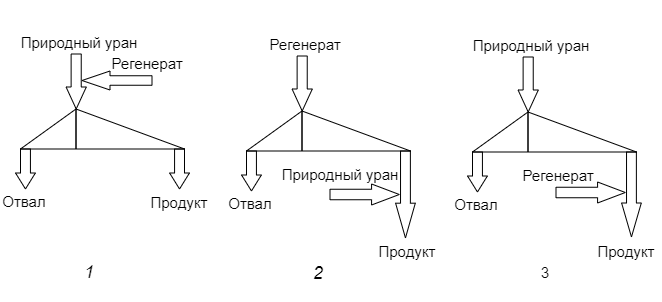
\includegraphics[scale=0.7]{cascades/diagram1}}
  \caption{Схемы на основе ординарного каскада}\label{fig:diagram1}
\end{figure}

Для всех вариантов схем рис. \ref{fig:diagram1} сотношение между расходом регенерата и разбавителем природного происхождения определяется пределом допустимой концентрации $^{232}$U в конечном продукте -- низкообогащенном уране. Также делается поправка на необходимость компенсации отрицательной реактивности $^{236}$U. В то же время концентрация $^{235}$U не должна быть ниже, чем требуется для НОУ с определенными свойствами.

Основным преимуществом таких схем является простота реализации, поскольку нет необходимости в модификации устройства каскада -- операции разбавления осуществляются за пределами  ординарного каскада. При этом, как недостаток можно выделить потери работы разделения, возникающие из-за смешения потоков с различными изотопными концентрациями $^{235}$U. 
Однако такие схемы не пригодны для решения задачи вовлечения регенерата в условияx многократного рецикла, как будет показано в данной диссертационной работе.

Рассмотрим вариант схемы, рис.\ref{fig:diagram1}.2, лучшим образом подходящий для задачи воврата регенерата урана второго рецикла (NET).

Схема рисунка \ref{fig:diagram1}.2 представляет собой возможный способ снижения накопления вредных изотопов в регенерате урана \cite{SposobIzotopnogoVosstanovleniyaa}. Разбавление осуществляют следующим образом: сначала из регенерата в ординарном каскаде получают высокообогащенный уран (ВОУ), который затем разбавляют смесью, не содержащей минорных изотопов, добиваясь нужного содержания изотопа $^{235}$U в финальном продукте-низкообогащенном уране. Например, таким разбавителем может быть природный уран или отвалы разделительного производства. Для обогащения по изотопу $^{235}$U перед последующим разбавлением предложена массовая концентрация $\approx$36\% \cite{SposobIzotopnogoVosstanovleniyaa}. Практическое использование данной схемы ограничивают следующие недостатки: 
\begin{enumerate}
  \item потери работы разделения при разбавлении ВОУ (количественные оценки величин затрат работы разделения для рассматриваемой схемы будут представлены в заключительном отчете по НИР).
  \item ухудшение радиационной обстановки из-за загрязненности разделительного оборудования примесными изотопами, в частности $^{232}$U, ухудшающим радиационную обстановку (смотри выше).
  \item необходимость обогащения материала до уровня высокообогащенного урана, когда концентрация изотопа $^{235}$U превышает 20\%. Такой подход может иметь ограничения со стороны регулятора -- обогатительный комбинат может быть не в праве нарабатывать материал с такой высокой концентрацией $^{235}$U -- ввиду режима нераспространения.
\end{enumerate}

Таким образом, рассмотрение приведенного ряда модификаций ординарного каскада подталкивает к дальнейшим поискам схем, которые бы нивелировали перечисленные недостатки.
Обзор таких каскадов "второго поколения" и будет предложен в двух последующих разделах.

\subsection{Усовершенствованные каскада с дополнительными внешними потоками (многопоточные схемы)}

\subsubsection{Применение дополнительных потоков питания}

Предожена схема с дополнительным потоком питания в виде регенерата, который подают на отдельную ступень рис. \ref{fig:2_inputs}) \cite{sulaberidzeQuasiidealCascadesAdditional2006}.
\begin{figure}[ht]
  \centerfloat{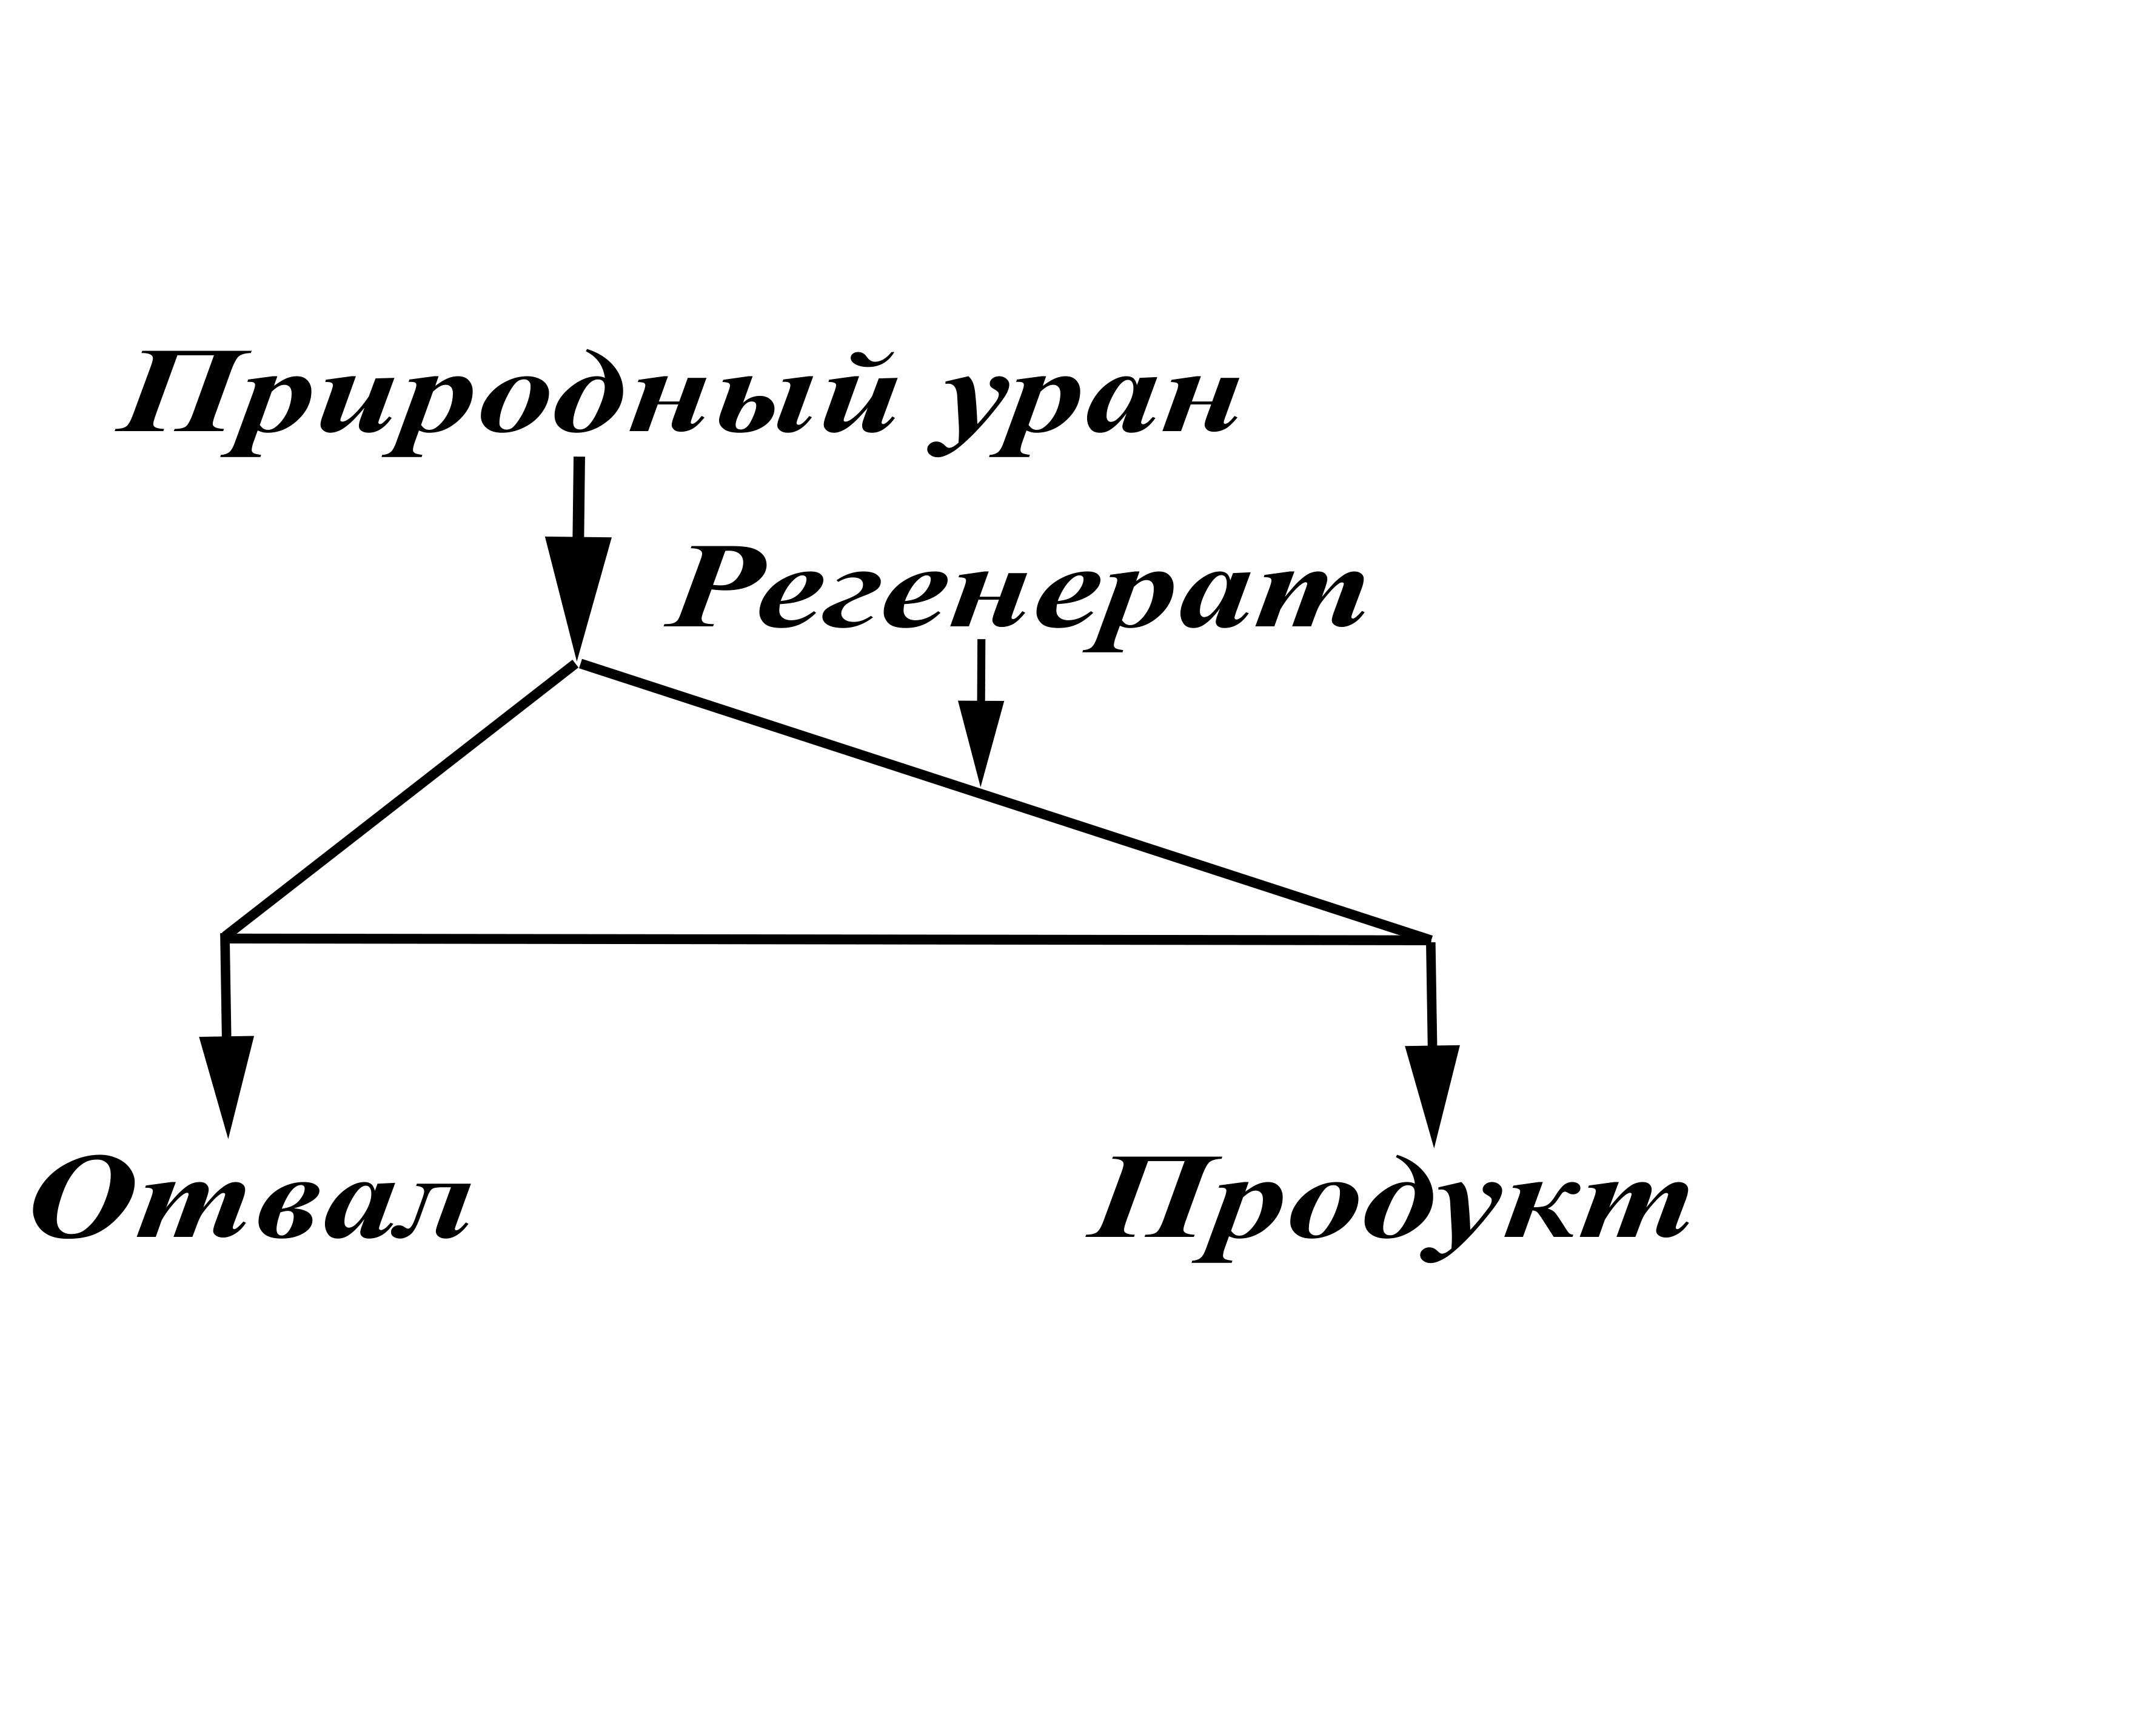
\includegraphics[scale=0.07]{cascades/2in}}
  \caption{Каскад с дополнительным потоком питания}
\end{figure}

Этот метод позволяет избежать потери работы разделения в ходе смешения потоков с различными концентрациями $^{235}$U, располагая дополнительный входной поток там, где концентрации внешнего и внутреннего потоков в $^{235}$U совпадают. Под внешними потоками следует понимать потоки, подаваемые в качестве питания каскада, а под внутренними -- потоки, циркулирующие внутри каскада. отсюда, преимущество схемы с дополнительным потоком питания по сравнению с предыдущими обычными схемами, связано с отсутствием потерь работы разделения \cite{smirnovKaskadnyeShemyZadachah2012, sulaberidzeQuasiidealCascadesAdditional2006}.

Однако общим недостатком всех вышеупомянутых схем (рис. \ref{fig:diagram1, fig:2_inputs}), является необходимость использования большого количества природного урана.
Вне зависимости от их устройства, для решения поставленной задачи, необходимо осуществлять разбавление регенерата существенным количеством природного урана, в несколько раз превышающим долю используемого регенерата. Это необходимо, прежде всего, чтобы снизить содержание $^{232}$U в продукте.
Тем не менее, при повторном использования топлива ВВЭР, даже такой подход может обеспечить значительную экономию природного урана $\approx$16\% уже на первом рецикле.
Применение же многократного рецикла, позволяет и дальше увеличивать экономию природного ресурса \cite{colemanEvaluationMultipleSelfrecycling2010}), как показано в оценках в \cite{smirnovEvolutionIsotopicComposition2012}.

Проблема необходимости обеспечивать питание каскада преобладающим количеством природного урана , чтобы, в сущности, "разбавлять" четные изотопы  $^{232,234}$U, содержащиеся в регенерате, идет бок о бок с невозможностью обеспечить условие "полного" возврата выгоревшего топлива в ЯТЦ.
Для рассмотренных схем, такое условие, заключающееся в использовании 1 кг ОЯТ на 1 кг НОУ продукта, достижимо только для изотопных составов первого (иногда второго) рецикла топлива легководного реактора.
Таким образом, с помощью такой схемы нельзя обеспечить заданую пропорцию вовлечения регенерированного урана в условиях многократного рецикла \cite{smirnovApplyingEnrichmentCapacities2018}.
На примере рассматриваемого каскада с двумя питаниями, начиная с третьего цикла, расходовать требуемый уровень регенерата становится невозможно из-за ухудшения изотопного состава урана и наличия ограничений на изотопы $^{232,236}$U.

Так, в \cite{smirnovApplyingEnrichmentCapacities2018} были рассчитаны экономия природного урана и работы разделения (РР) и показано, что для каждого цикла можно достичь $\approx$20\% экономии природного урана до того, как к третьему циклу повторного использования происходит значительная деградация изотопного состава.
Чтобы повысить пределы экономии природного урана, необходимо искать альтернативный разбавитель. Например, это может быть обедненный уран (так называемые «хвосты» (или отвалы) -- побочный продукт процесса обогащения). Это может быть плодотворно использовано для частичной замены природного урана в качестве основного разбавителя, хотя этот материал часто рассматривается как «отходы». Такая конфигурация изображена на рис. \ref{fig:3_inputs}, где $F_{1}, F_{2}, F_{3}$ -- потоки питания в виде ОГФУ, природного урана и регенерата, соответственно; W, P -- потоки отвала и питания. Описание математической модели приведено в \cite{smirnovEnrichmentRegeneratedUranium2014}.

Такой подход предполагает снижение содержания $^{235}$U во вновь образовавшемся ОГФУ, по сравнению с исходным, и требует исследования перспектив дальнейшего использования такого материала в бланкетах реакторах-бридерах. Такой дважды обедненный ОГФУ, к тому же содержащий минорные изотопы, по-видимому должен быть первым на очереди к переработке в установках типа «W-ЭХЗ».

\begin{figure}[ht]
  \centerfloat{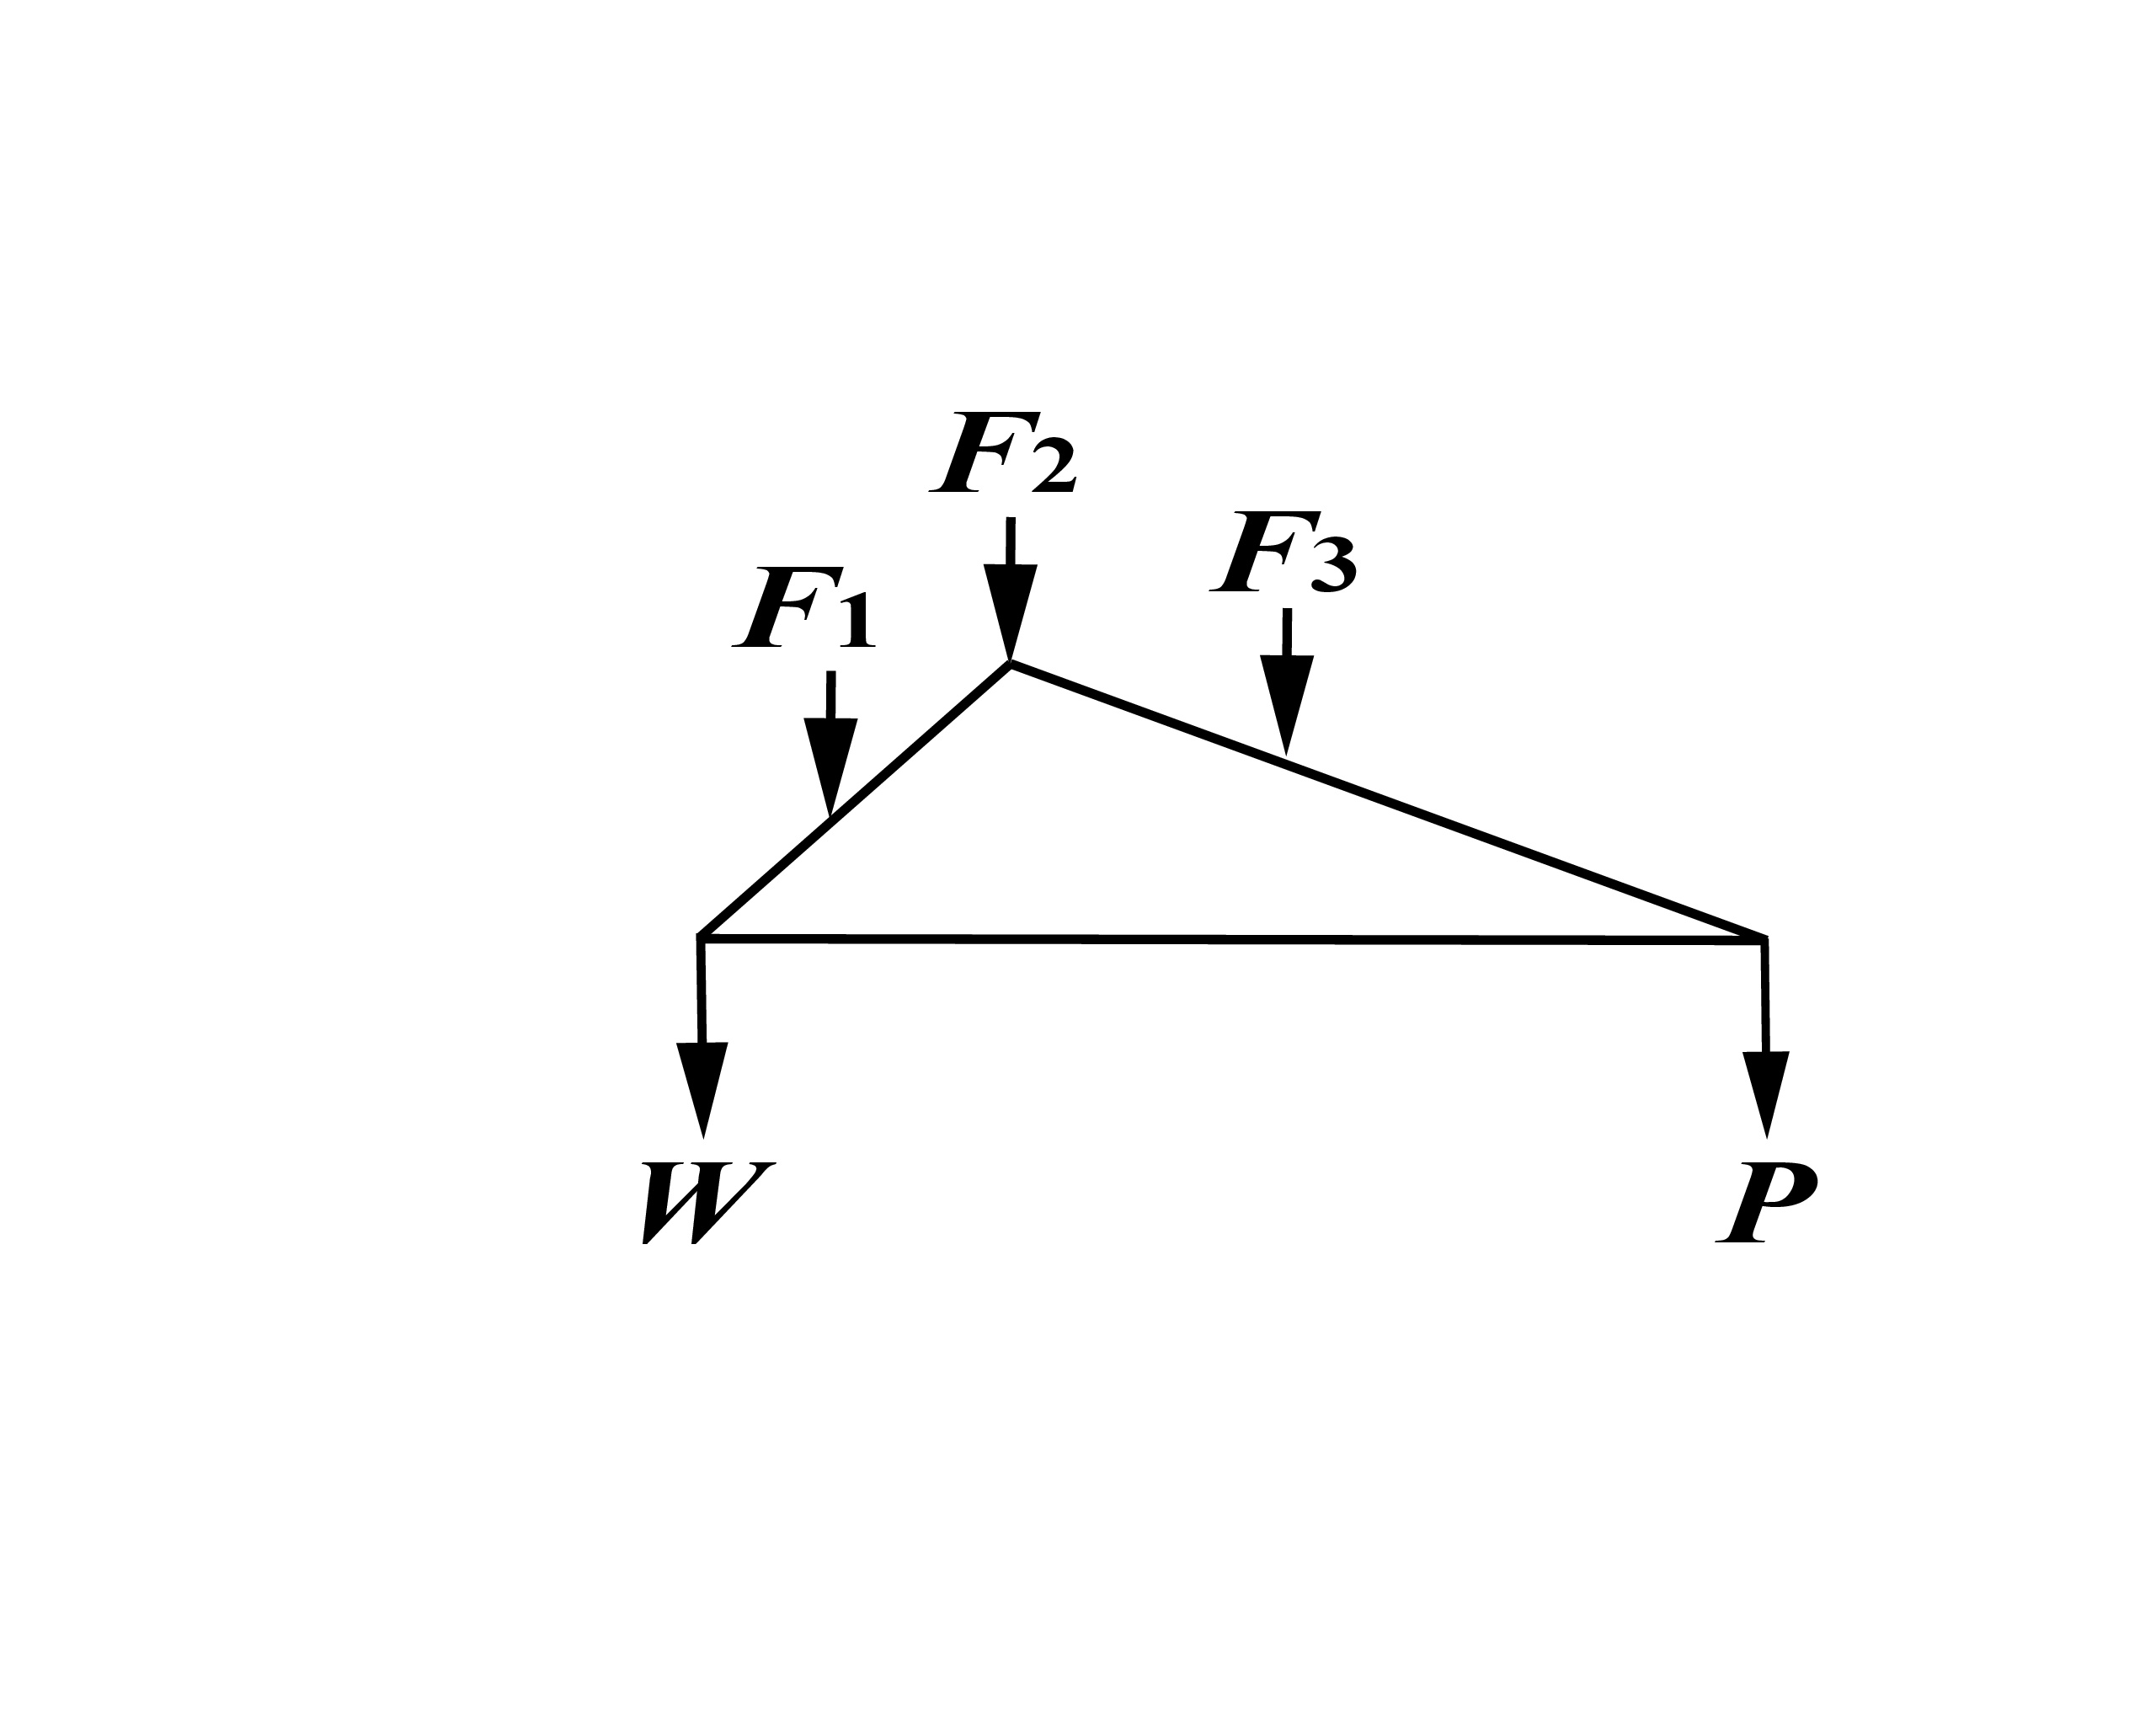
\includegraphics[scale=0.17]{cascades/3in}}
  \caption{Каскад с тремя потоками питания}\label{fig:3_inputs}
\end{figure}

Основным преимуществом использования каскада рис. \ref{fig:3_inputs} является возможность б'ольшей экономии природного урана.
В \cite{smirnovApplyingEnrichmentCapacities2018}, например, демонстрируется устойчивая экономию половины природного урана на каждом рецикле. Следует отметить, что этот эффект достигаетс ценой дополнительного расхода РР. При этом возможен выбор соотношения разбавителей и, что позволяет регулировать экономию природного урана и перерасход РР.
Эта особенность позволяет «настраивать» каскад для достижения компромисса между этими антагонистическими показателями.
Такой прием позволяет добиваться оптимального по себестоимости баланса затрат на эти два основных конкурирующих показателя.
Заметим, что в качестве критериев для выбора оптимальной схемы как правило и используют минимизацию работы разделения и расхода природного урана для получения единицы товарного НОУ. Эти характеристики, в основном, и определяют величину удельных затрат на получение коммерческого продукта.

Кроме этого, вариант рис. \ref{fig:3_inputs} полезен для решения проблемы утилизации накопленных объемов обедненного урана \cite{smirnovEnrichmentRegeneratedUranium2014}. Поскольку гексафторид урана является агрессивным веществом, его хранение связано с затратами, и емкости для хранения следует время от времени заменять из-за коррозионных процессов \cite{fitchOPTIONSDISPOSALREAPPLICATION2009, oecdManagementDepletedUranium2001}.

Итак, исходя из результатов работы \cite{smirnovApplyingEnrichmentCapacities2018}, схема (рис. \ref{fig:3_inputs}), как и схема рис. \ref{fig:2_inputs}, позволяет обеспечить полный возврат урана в ядерный топливный цикл только для двух первых циклов повторного обращения.
При заданных в работе \cite{smirnovApplyingEnrichmentCapacities2018} условиях, это невозможно для серии последовательных циклов из-за быстрого накопления вредных четных изотопов. При  этом отсутствует возможность с помощью такой схемы очистить смеси от этих нежелательных компонентов \cite{smirnovApplyingEnrichmentCapacities2018}.

Таким образом, возникает проблема очистки изотопных составов от четных изотопов, которые имеют тенденцию накапливаться от рецикла к рециклу, приводя к деградации изотопного состава.
Важность сдерживания накопления $^{232}$U при многократном переиспользовании была показана в работе \cite{smirnovEvolutionIsotopicComposition2012}.
Введение ограничения на $^{232}$U позволяет замедлить рост концентрации $^{236}$U в изотопном составе рециклируемого топлива.

Однако, как было отмечено, во всех рассмотренных схемах заметное снижение содержания изотопов $^{232,234,236}$U в финальном НОУ достигается, прежде всего, за счет разбавления регенерата внутри каскада смесями, полученными из урана природного состава (НОУ, ОГФУ, или сам природный уран).

Отсюда возникает вопрос отделения вредных $^{232,234,236}$U из изотопного состава рециклируемого материала.

В качестве дополнительного аргумента для поиска альтернативных каскадов, позволяющих выводить из системы $^{232,234,236}$U, приведем следующий факт.
В последнее время конструкция ВВЭР развивалась к увеличению максимального выгорания топлива (до 70 МВт-день / кг U в ВВЭР-1200) \cite{asmolovNewGenerationFirstofthe2017}, с целью снижения стоимости топливной составляющей \cite{andrianovaPovyshenievygoraniyaToplivaVVER2008}.
Имея ввиду, что, согласно природе цепной реакции, рост остаточного содержания $^{232,234,236}$U пропорционален уровню выгорания \cite{VeryHighBurnups2006}, схемы, нацеленные на очистку $^{232,234,236}$U заслуживают особого внимания.

Далее будут представлены способы, с помощью которых можно частично удалить нежелательные изотопы из системы. Это может быть сделано с помощью схем, которые позволяют извлекать промежуточный продукт, или с помощью составных схемам (несколько последовательных каскадов, например, двойной каскад). Остановимся на первых поподробнее.

К тому же, в случае успеха в продвижении российских услуг по реконверсии RepU на мировой рынок, очистка от $^{232}$U может быть востребована в силу ограничения лицензии российского оператора ($5\cdot10^{-7}$\% (5ppb) по $^{232}$U), если не будут применены иные способы улучшения изотопного состава.
Однако существуют практики возврата регенерата в ЯТЦ, для которых проблема очистки регенерата от четных $^{232,234}$U не актуальна вне необходимости многократного рецикла. Так, Французская электроэнергетическая компания EDF выбрала стратегию прямого обогащения регенерированного урана. Такой подход воплощен на АЭС Cruas, которая имеет лицензию на работу с топливом, в котором ограничение содержания $^{232}$U в 6 раз выше ограничения, принятого в РФ, и составляет 30 ppb.

\textcolor{red}{В презентации Щелканова с семинара ТВЭЛ, ASTM C996 ограничивает присутствие $^{232}$U на уровне $5\cdot10^{-6}$\%, а в презентации от TENEX -- 5 ppb, то есть $5\cdot10^{-7}$\%.}

\subsubsection{Применение дополнительных потоков отбора}
Схемы, называемые каскадами с промежуточным продуктом были предложены с целью «очистки» от балластных изотопов (рис. \ref{fig:3_out}) \cite{palkinAnaliticheskiyRaschetSoderzhaniya2007}.Здесь в качестве основного продукта получают НОУ требуемых характеристик, а в качестве промежуточного продукта получают композицию с пониженным содержанием нежелательных изотопов.
\begin{figure}[ht]
  \centerfloat{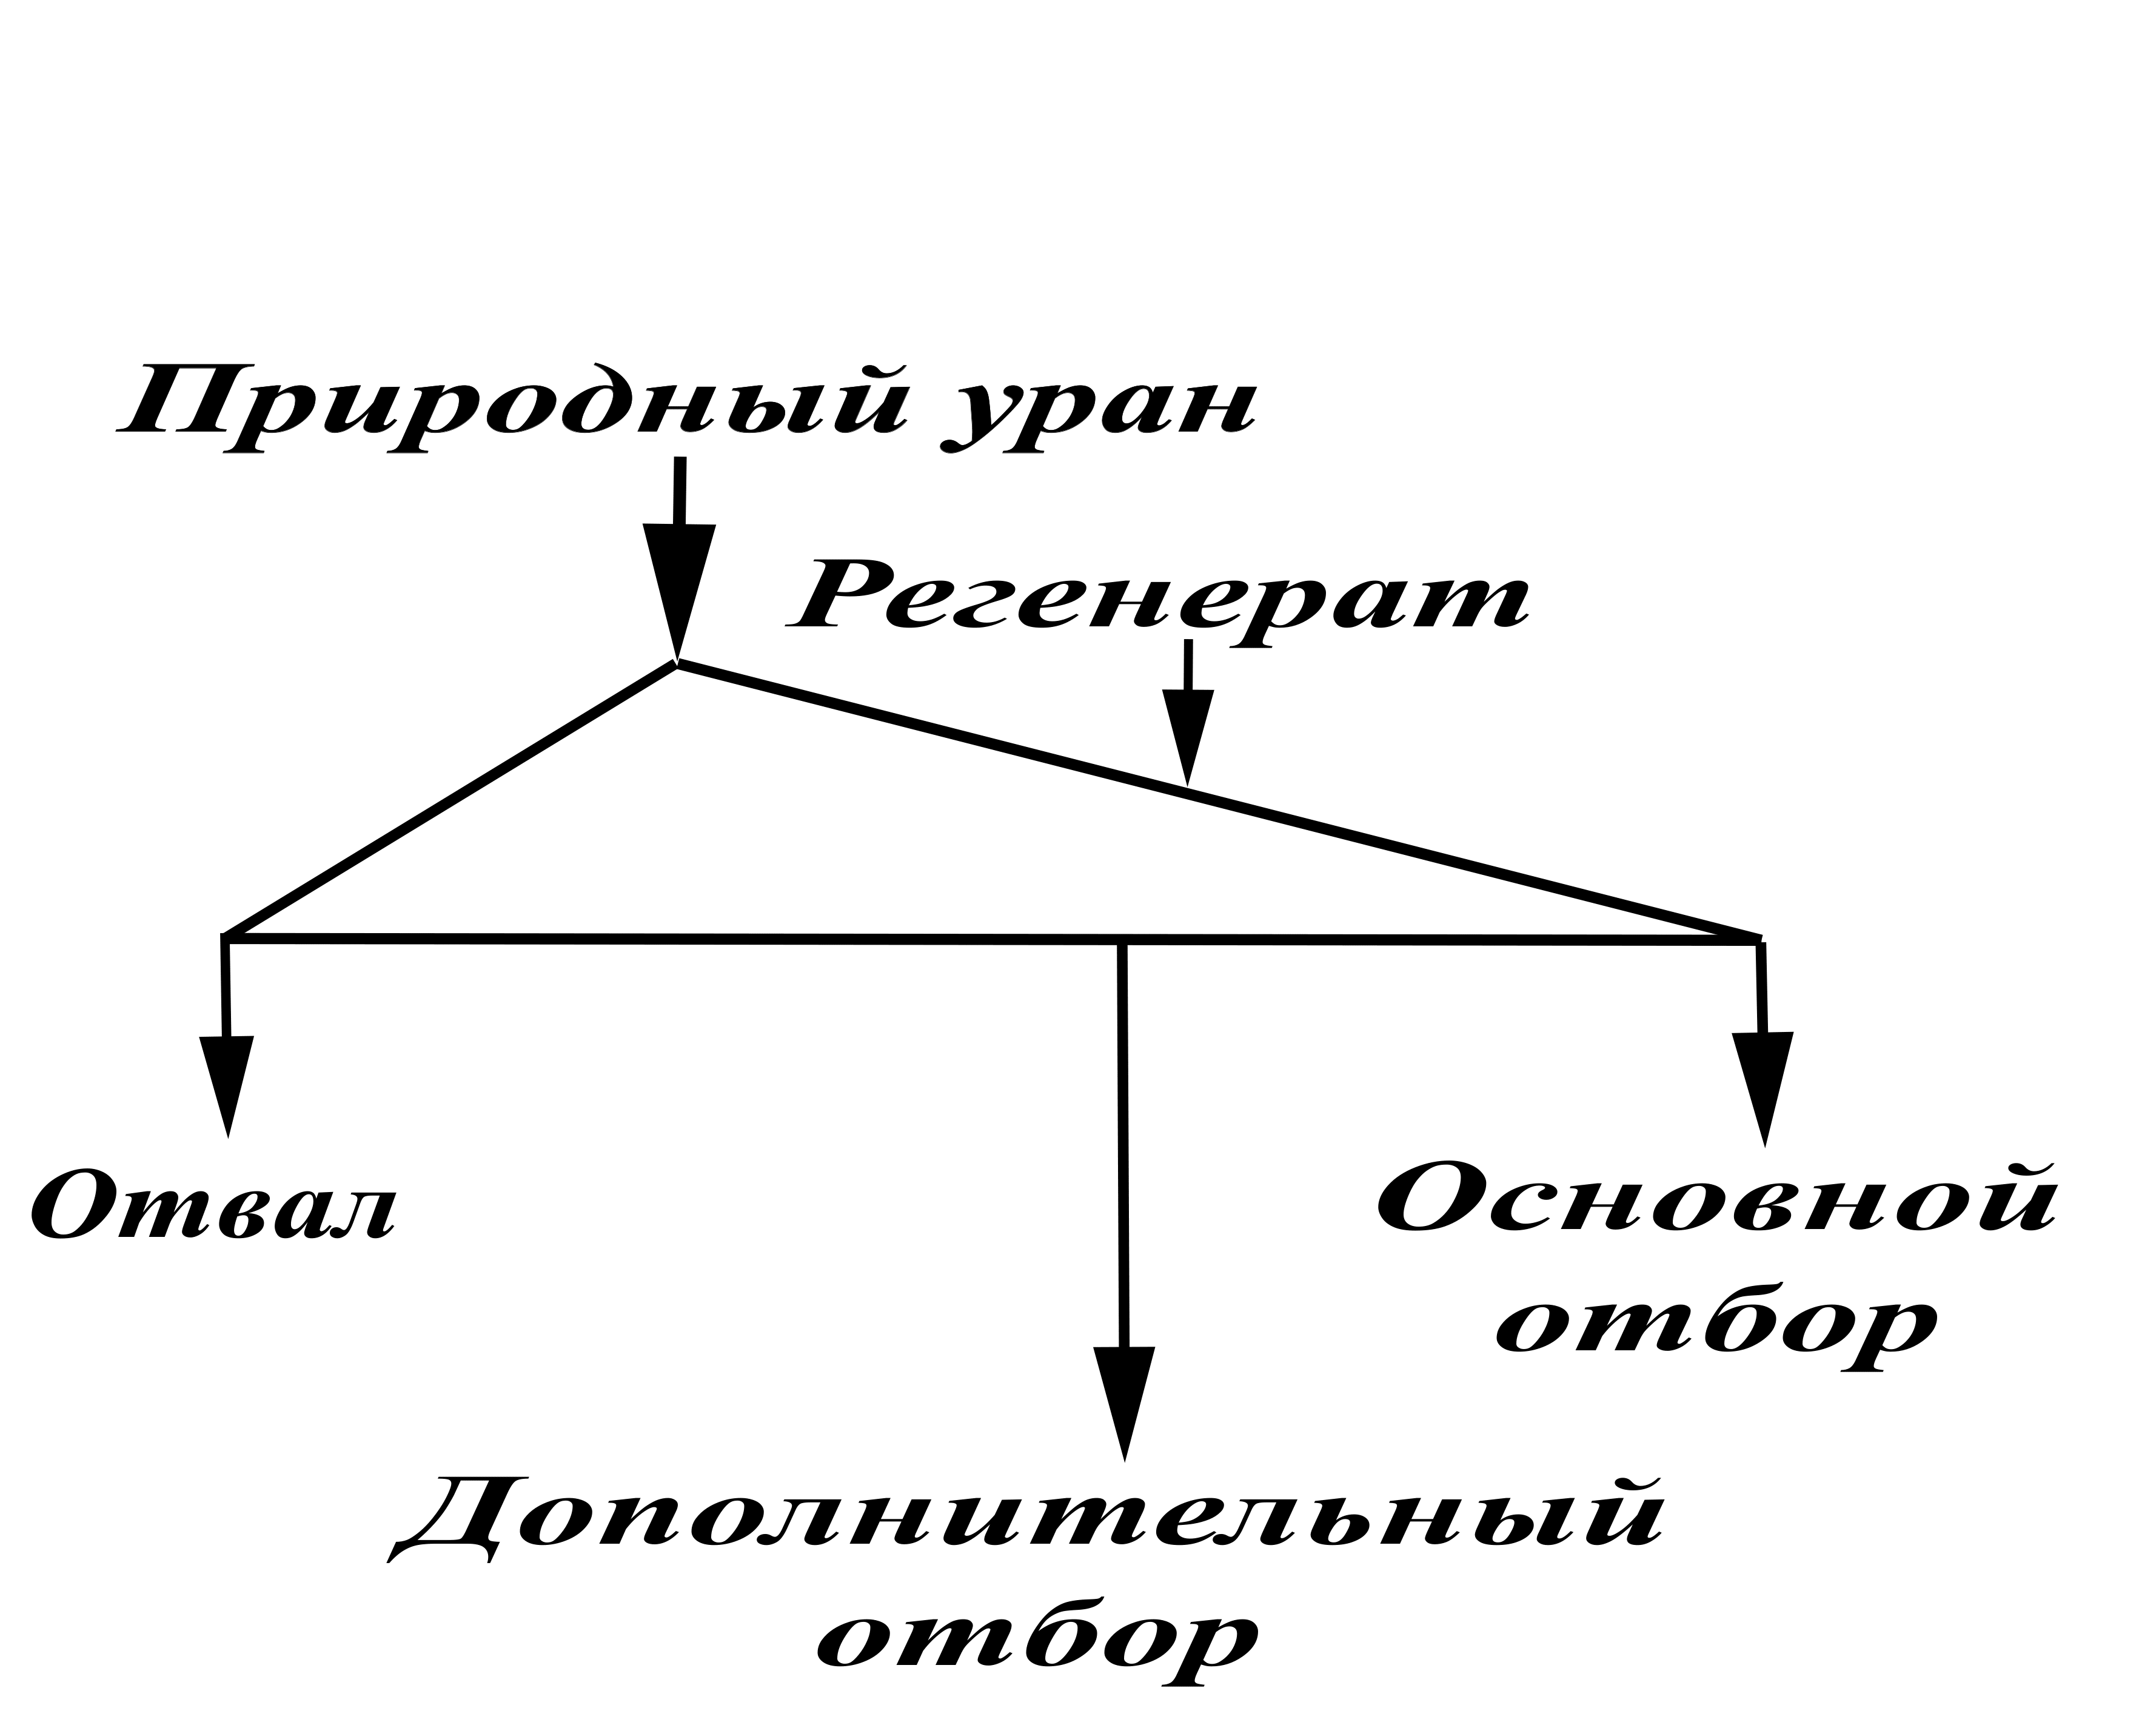
\includegraphics[scale=0.07]{cascades/3out}}
  \caption{Каскад с дополнительным потоком отбора}\label{fig:3_out}
\end{figure}

Частичное удаление из смеси более четных изотопов на первой стадии, позволяет получить больше преимуществ от увеличения количества делящегося $^{235}$U на второй -- при ее обогащении до товарного НОУ \cite{palkinSeparationUraniumIsotopes2010}.
Концентрация $^{235}$U в этом "очищенном" продукте составляет примерно 0,8--1,1 от его значения в исходном регенерате и регулируется как соотношением входящих потоков, так и положением промежуточной (дополнительноой) точки выходящего потока.
Как показано в \cite{palkinSeparationUraniumIsotopes2010}, в результате очистки содержание всех вредных изотопов значительно снижается. После чего, низкообогащенный уран с концентрациями $^{232,234,236}$U, удовлетворяющими требования ASTM для коммерческого продукта, может быть получен из очищенного промежуточного продукта путем его прямого обогащения \cite{shopenSposobPolucheniyaRazbavitelya2008}.
При этом важно заметить, что основной продукт НОУ каскада-очистителя также соответствует этим требованиям \cite{palkinSeparationUraniumIsotopes2010}. Следует отметить, что высокое качество очищенного регенерата достигается при малой доле потока регенерата, относительно природного урана, в случае, когда необходимо выполнить требования к каждому из производимых НОУ.
Основным преимуществом здесь является то, что эта схема, обеспечивающая одновременное снижение $^{232,234,236}$U, практически не теряет РР и не требует загрязнения дополнительного каскада (будет обсуждаться далее в разделе составных схем).

Однако, важно отметить, что ввиду необходимости использовать в несколько раз большую доли природного урана в питании, этот каскад является по-существу схемой разбавления регенерата. 

Недостатки здесь заключаются в том, что эффект очистки обусловлен, прежде всего, уменьшением объема потока очищенного промежуточного продукта. Эффекта заметного снижения содержания минорных изотопов в дополнительном отборе можно добиться лишь при сильном разбавлении регенерата природным сырьем, в соотношениях, лежащих в диапазоне (1-25)/100 \cite{palkinSeparationUraniumIsotopes2010, smirnovKaskadnyeShemyZadachah2012}. Следовательно, данная схема не может обеспечить широкомасштабного возврата регенерированного урана в топливный цикл ВВЭР, ввиду малой удельной экономию природного урана.  Более того, такой подход демонстрирует снижение экономии природного урана. Кроме того, такой подход демонстрирует снижение экономии природного урана, и не позволяет вернуть весь ОЯТ (в соотношении к продукту 1:1).
В качестве материалов, которые необходимо очистить посредством такой схемы, можно рассматривать составы загрязненного урана природного состава, «хвостов» процесса обогащения и других, «загрязненных» урановыми $^{232,234,236}$U \cite{palkinSeparationUraniumIsotopes2010}. 




\subsection{Комбинации нескольких каскадов (составные схемы)}\label{sec:ch1/sec2.3}
Под составными схемами подразумеваются различные вариации коммутации одиночных каскадов в единую составную структуру.

Рассмотрим принципы работы простейшего варианта составного каскада -- двойного каскада (рис. \ref{fig:double_ru}). Эта модификация направлена на эффективное удаление $^{232}$U из каскада и нацелена на получение НОУ реакторного качества без необходимости вовлечения природного урана \cite{SosninYuChelcov, TehnicheskieResheniyaPo, SposobIzotopnogoVosstanovleniya}.
Рассмотрим принципы работы такой схемы.
В первом каскаде (верхнем) $^{235}$U обогащается по легкой фракции (отбор первого каскада на рис. \ref{fig:double_ru}), где также накапливается $^{232}$U.
Затем, эту смесь направляют во второй каскад, где самые легкие изотопы $^{232,234}$U концентрируется в загрязненной "отборной" части и выводится из обращения.
В то же время НОУ-продукт с требуемым уровнем обогащения по $^{235}$U направляется с тяжелой фракцией к другому выходу, в этой конфигурации представляющим из себя поток продукта.
\begin{figure}[ht]
  \centerfloat{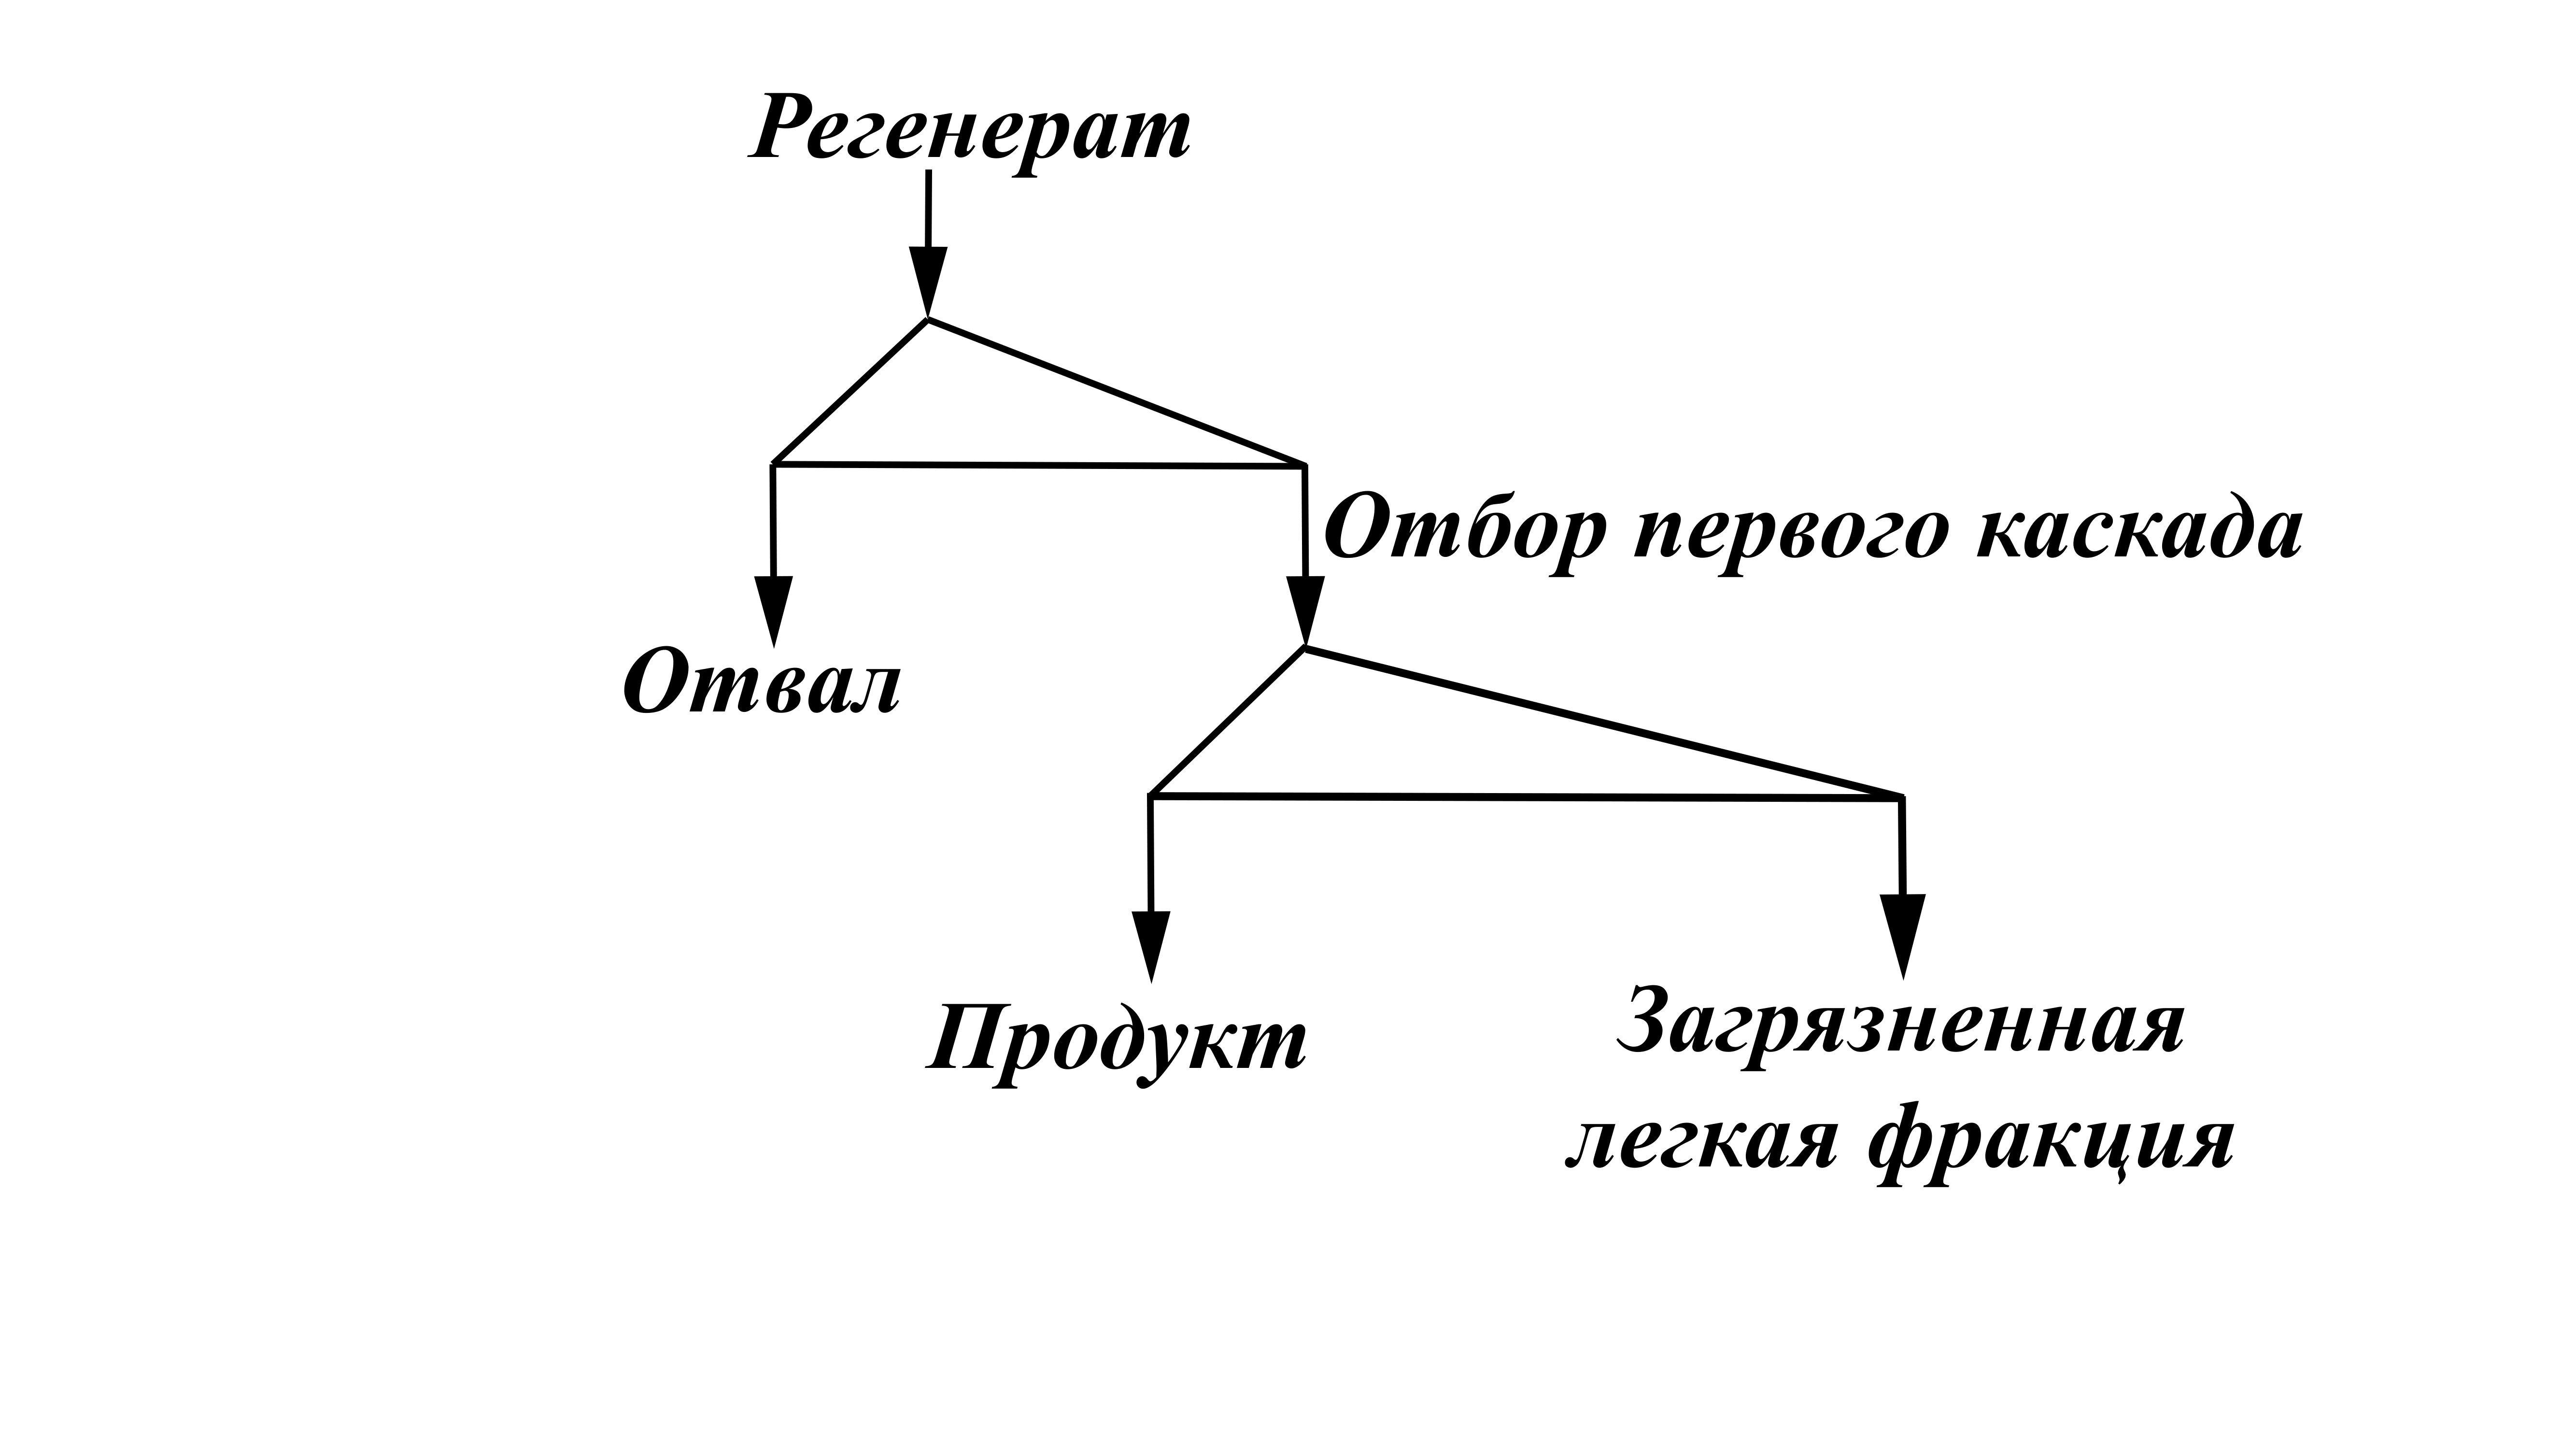
\includegraphics[scale=0.07]{cascades/double_ru}}
  \caption{Двойной каскад}\label{fig:double_ru}
\end{figure}

Рассмотрим физический эффект, который происходит в легком конце второго каскада, на котором необходимо сконцентрировать вредные четные изотопы.
При доведении концентрации $^{235}$U до уровня, свойственного оружейному материалу, наблюдается разворот кривой монотонно возрастающей концентрации $^{235}$U, тогда как прекращение обогащения смеси по $^{232,234}$U (а также $^{233}$U, который учитывается не во всех рассмотрениях, например Палкиным (как это аккуратно объяснить?)) не происходит.

Таким образом, этот с помощью этого приема во втором каскаде осуществляется пространственное разделение легкой фракции с $^{232,233,234,235,236}$U и тяжелой с $^{235,236,238}$U.
Как результат, возможность удалять из изотопной смеси легкие четные изотопы связана с потерями ценного $^{235}$U в выводимом потоке.
К тому же, такой материал классифицируется как высокообогащенный уран. А так материал такой категории считается крайне ценным, возникает вопрос о целесообразности его окончательной утилизации. 

В некоторых случаях такая схема подразумевает использование газа-носителя (или буферного газа) \cite{prusakovCorrectingIsotopicComposition2008, SposobIzotopnogoVosstanovleniyab}.


Использование буферного газообразного соединения, которое является инертным (неактивным) к гексафториду урана -- рабочему газу, позволяет повысить эффективность отделения $^{232}$U из переработанного урана и уменьшить потери $^{235}$U. Идея применения этого газа с массовым числом, близким к $^{232}UF_6$, была выдвинута в \cite{SosninYuChelcov}, исходя из предположения, что такой газ мог бы служить матрицей-носителем для $^{232}UF_6$. В этом исследовании авторы предложили использовать фреон, поскольку среднее массовое количество этого соединения практически совпадает с массовым числом $^{232}UF_6$ (и ниже, чем в $^{235}UF_6$, что немаловажно).
Среди недостатков рассматриваемой схемы:
\begin{enumerate}
  \item оба каскада в схеме загрязнены изотопом $^{232}$U, что осложняет радиационную обстановку на разделительном производстве.
  \item в предлагаемой схеме принципиально отсутствует возможность снижения накопления изотопа $^{236}$U, негативное влияние которого на размножающие характеристики тепловыделяющих сборок (ТВС) требует дополнительного обогащения по изотопу $^{235}$U. При этом эквивалентная концентрация $^{235}$U может быть заметно больше, чем в штатном топливе, что обуславливает дополнительные затраты работы разделения.
  \item для опции с газом-носителем, получаемый товарный продукт необходимо очищать от этого газа, что, очевидно, также приводит к увеличению удельных затрат.
\end{enumerate}

Таким образом,  вариант без буферного газа предпочтительным, поскольку в ходе технологического процесса не возникает необходимости очищать смесь от буферного газа \cite{smirnovKaskadnyeShemyZadachah2012}. Среди недостатков таких схем следует отметить, что получение высокообогащенного урана с содержанием $^{235}$U более 20\%, что усложняет проблему соответствия международным стандартам обращения с делящимися материалами.
Такой подход помогает повторно обогащать переработанный уран, даже не разбавляя его сырьем, что делает его наилучшим вариантом с точки зрения экономии природного газа. Однако этот двойной каскад не может обеспечить решение проблемы "полного" (1:1) возврата. Она расходует значительно больше необходимого $\approx$0,93 кг регенерата на производство 1 кг свежего НОУ. Это означает, что для загрузки реактора, в котором используется переработанное топливо, необходимо будет использовать другой источник, скорее всего, таким ресурсом будет природный уран. Следовательно, в контексте закмыкания ЯТЦ по урановой составляющей и возврата в рассматриваемый реактор всего объема топлива, реальная экономия природного урана будет не 100\%, а в несколько раз меньше -- лучшем случае 15-20\%. И, как уже упоминалось, подобный принцип может быть реализован на практике без дополнительного агента -- газа-носителя.

В \cite{palkinPurificationReprocessedUranium2016} подчеркивается, что, тогда как в первом же каскаде достигается концентрация > 20\% от $^{235}$U, которая затем во втором каскаде еще больше повышается в потоке, уносящем "загрязненную" фракцию, такая мера едва ли заслуживает одобрения из-за строгих правил производства ВОУ во всем мире \cite{ManagementHighEnriched2005}.

В качестве необходимой модификации двойного каскада была предложена альтернативная каскадная схема, которая в принципе позволяет решить проблему полного возврата регенерата в цикл. В качестве такой альтернативы на рис. \ref{fig:triple} изображен случай, когда первый каскад, как и на схеме рис. \ref{fig:double_ru} увеличивает концентрацию $^{235}$U со всеми более легкими изотопами и направляет их (через выходящий поток в правой части на рисунке) ко второму каскаду, который будет концентрировать $^{232,234}$U в потоке загрязненного продукта \cite{smirnovObogashchenieRegenerirovannogoUrana2018}. Хотя на этот раз композиция тяжелой фракции на выходе из второго каскада разбавляется предварительно подготовленным НОУ для контроля концентраций $^{232,234}$U в допустимых пределах и для управления соотношением рециркулируемых материалов (для поддержания требуемого уровня возврата регенерата в ядерный топливный цикл).
\begin{figure}[ht]
  \centerfloat{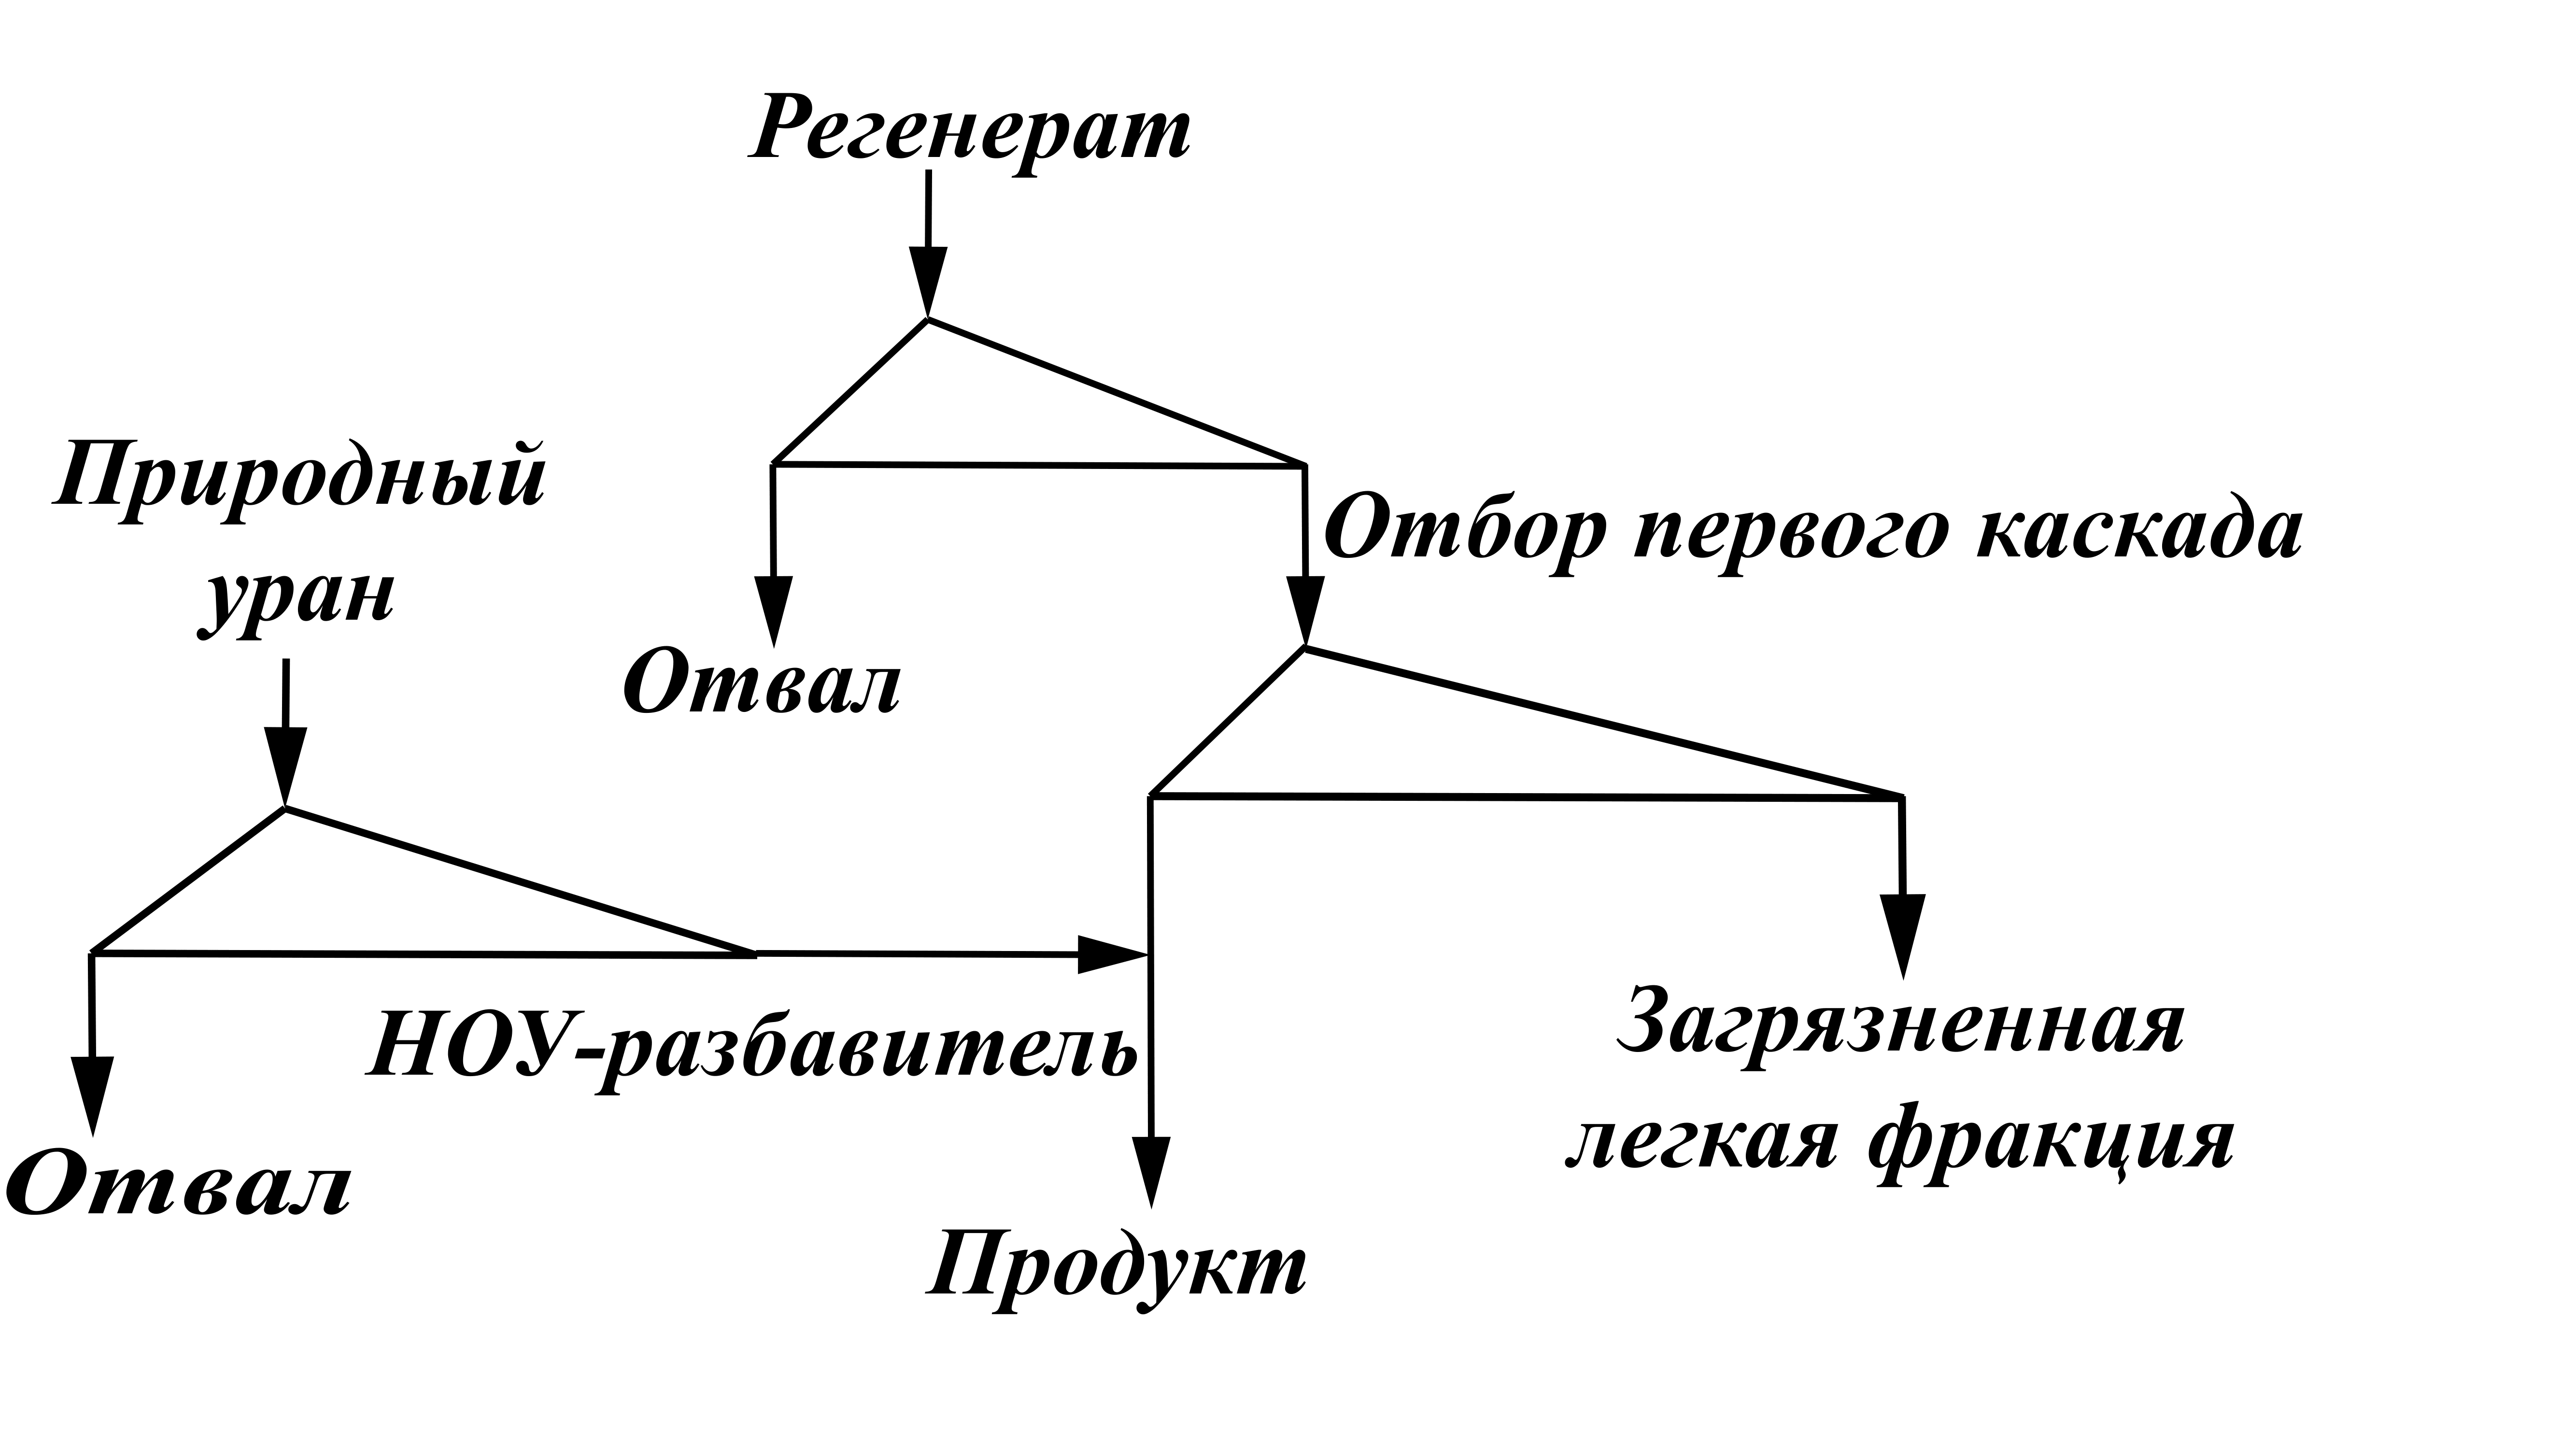
\includegraphics[scale=0.07]{cascades/triple}}
  \caption{Тройной каскад}\label{fig:triple}
\end{figure}

Хотя этот вариант и кажется идеальным, цена хранения побочного продукта из загрязненной смеси слишком высока, что мгновенно делает схему нежизнеспособной, если нет способов избежать такого негативного побочного эффекта.
Однако в \cite{smirnovMethodEnrichReprocessed2019} автор предложил применить дополнительный каскад для производства НОУ из загрязненной смеси, сильно разбавленной обедненным ураном (которые имеют высокую концентрацию $^{235}$U ~ 20\%), чтобы получить конечный продукт в двух исходящих потоках и достичь значительной экономии природного урана (~ 38\%) даже для «грязной» композиции, которая уже была переработана пять раз. Расчеты показали, что такой подход позволяет производить НОУ коммерческого качества, расходуя должное количество переработанного урана, в то же время отвечая стандартным спецификациям $^{232}$U (и условиям, установленным для других четных изотопов). В то же время, предлагаемая схема обеспечивает более существенную экономию природного урана, чем большинство схем обогащения переработанного урана. Это могло бы также обеспечить широкомасштабную «мобилизацию» обедненного урана.
Как мы видим, такие схемы также очень ценны как инструмент для возврата в ЯТЦ требуемого количества переработанного урана.

\subsubsection{Другие варианты реализации}

Существует конфигурация двойного каскада (рис. \ref{pure_double}), где предлагается использовать прием смещения точки подачи питания в сторону точки отбора легкой фракции \cite{sulaberidzeProblemsRefinementRecycled4}. При этом в \cite{palkinReprocessedUraniumPurification2013} отмечается, что это позволяет добиться существенного снижения доли $^{232}$U в конечном продукте. Однако, такой вариант связан с существенными потерями работы разделения и не позволяет осуществлять эффективную очистку от $^{234,236}$U \cite{palkinPurificationReprocessedUranium2016}.
\begin{figure}[ht]
  \centerfloat{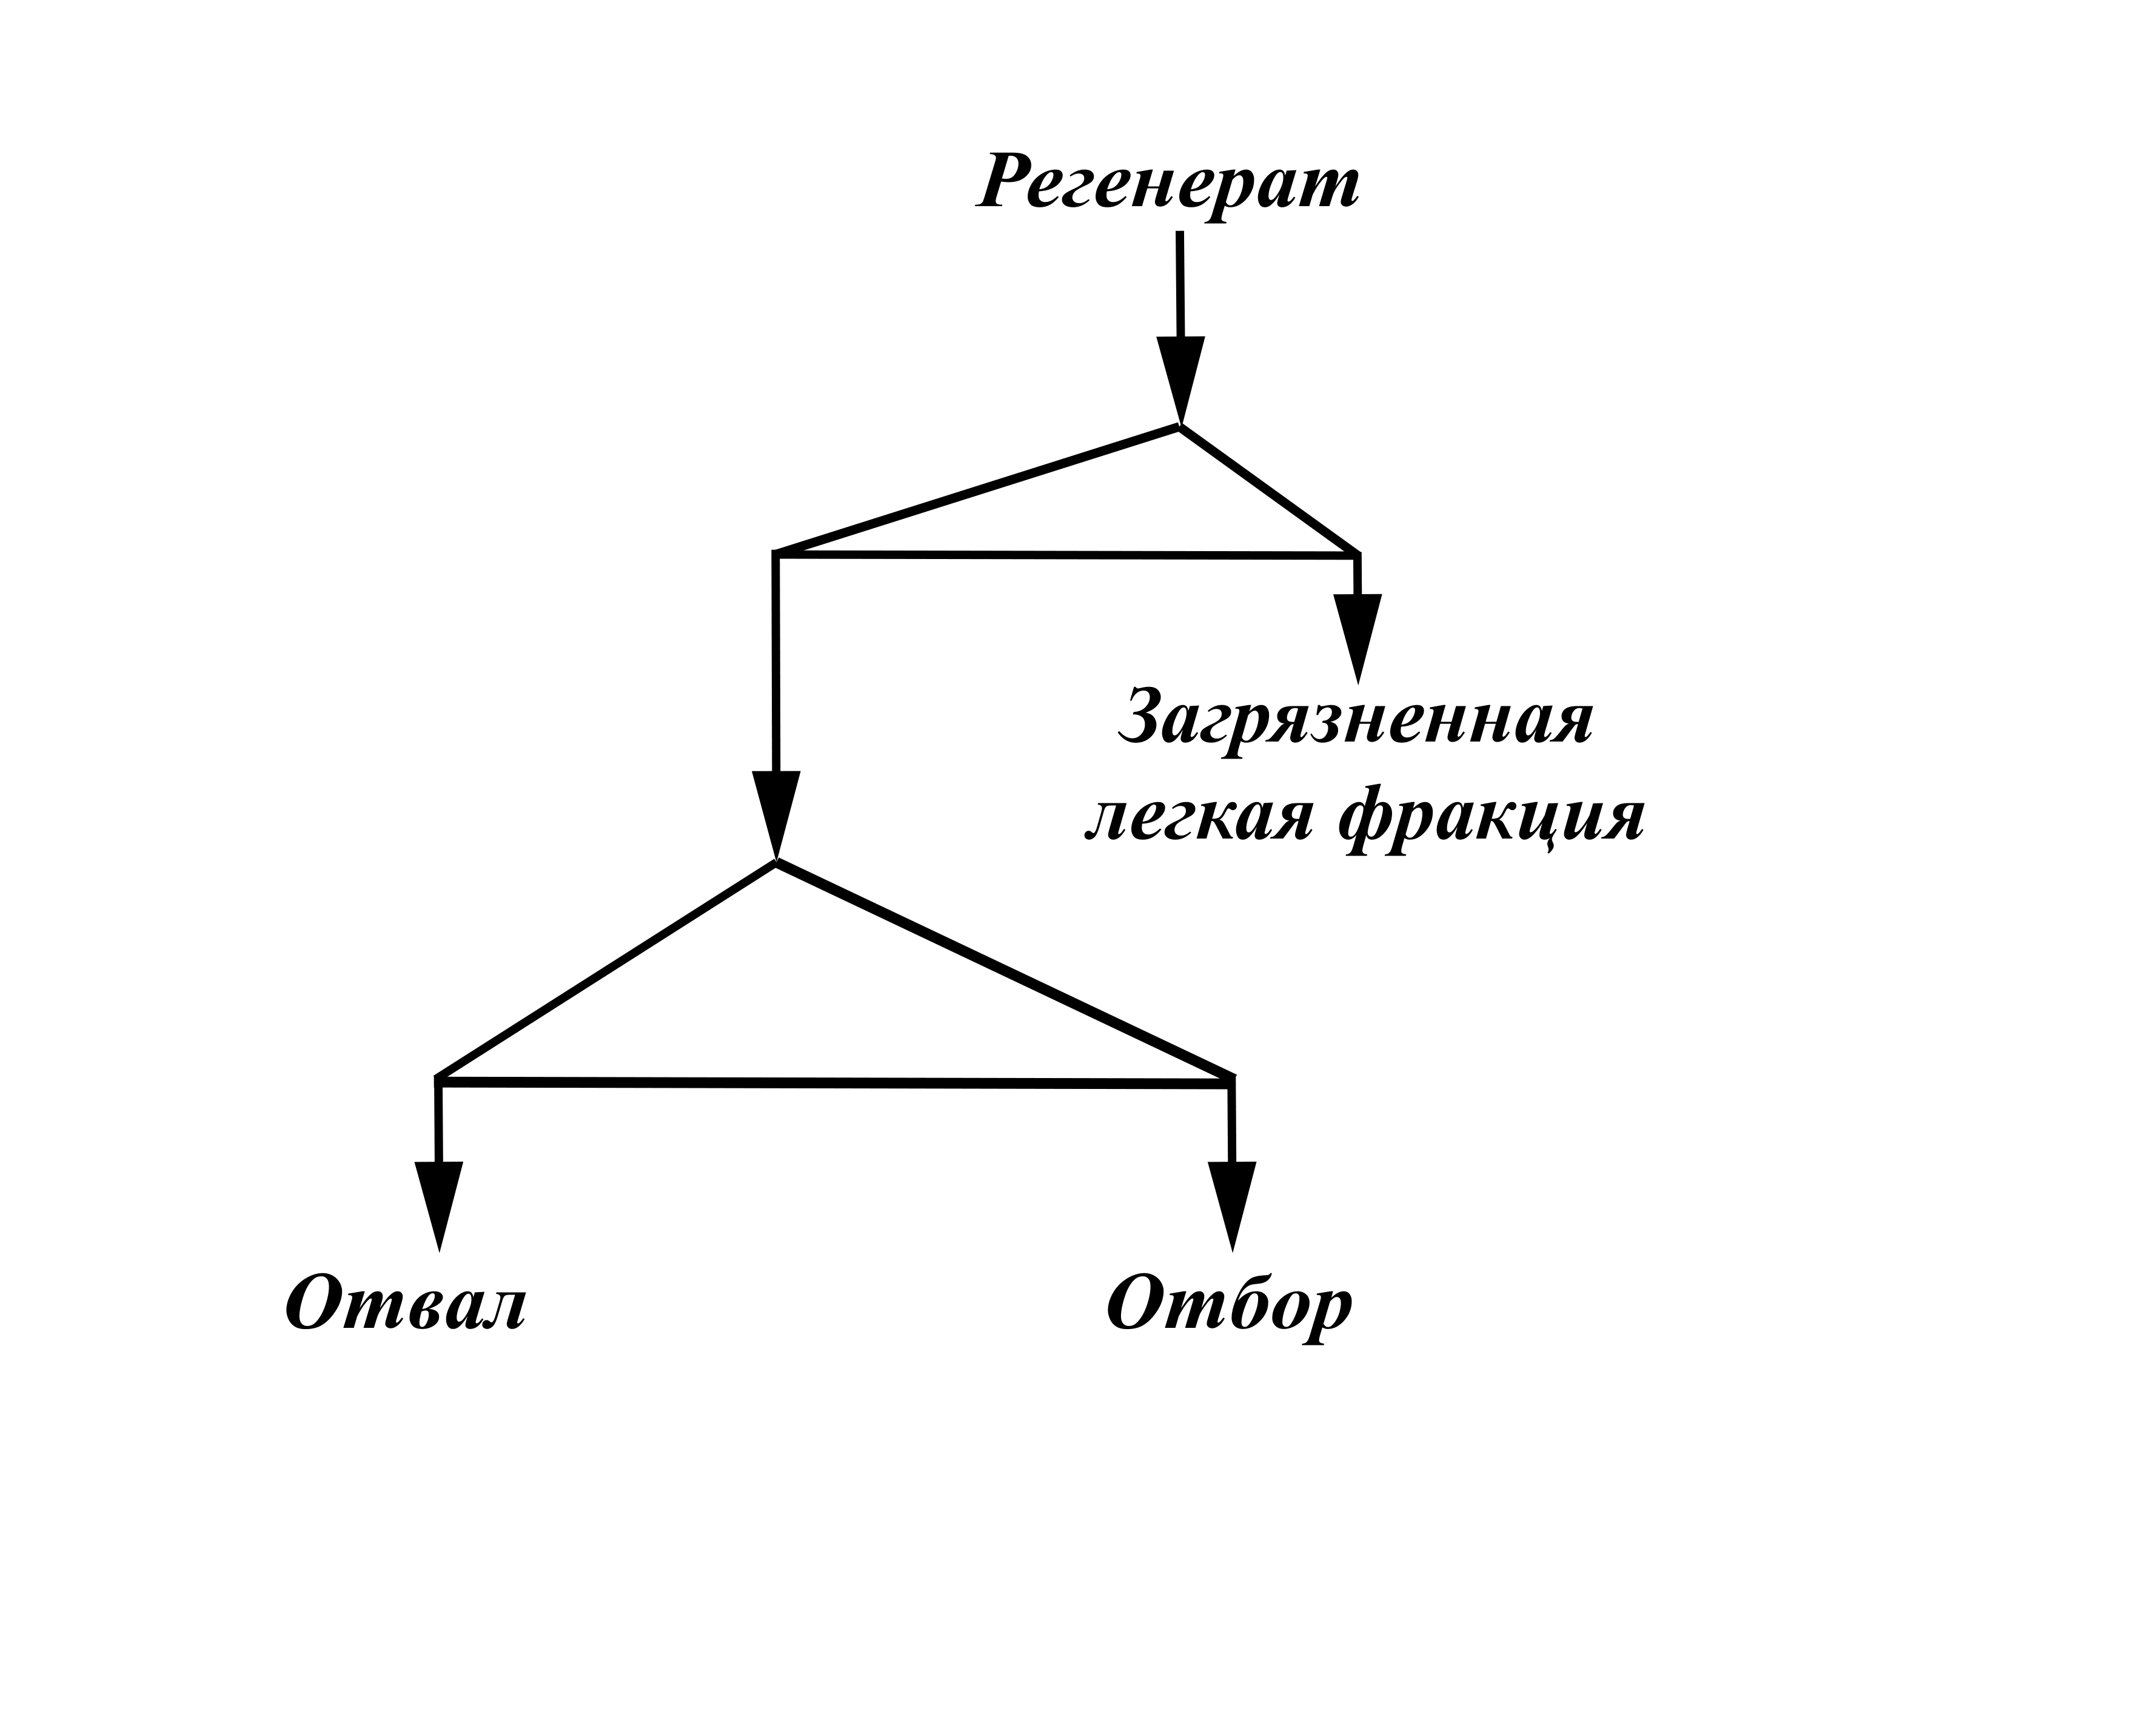
\includegraphics[scale=0.1]{cascades/pure_double}}
  \caption{Тройной каскад}\label{fig:pure_double}
\end{figure}

Рассмотрим другие способы коммутации каскадов в составные схемы из различных видов единичных каскадов.

В работе \cite{palkinPurificationReprocessedUranium2016}, представившей схему рис. \ref{fig:int_double}, в первом в последовательности каскаде в качестве промежуточного продукта -- в каскаде с дополнительным выходящим потоком в виде очищенного регенерата -- получена изотопная композиция с пониженной концентрацией самого легкого изотопа --  $^{232}$U. Затем такой очищенный полупродукт поступает в обычный каскад, как показано на рисунке \ref{fig:int_double}, где он обогащается до необходимого уровня по $^{235}$U. Кстати, основной продукт первого каскада также может удовлетворять заданным свойствам коммерческого НОУ. Вдобавок, автор данной работы подчеркивает возможность значительного снижения нежелательной концентрации $^{236}$U в случае уменьшения потока дополнительного отбора. Автор рекомендует применять этот эффект следующим образом: например, снизить концентрации  $^{234}$U и  $^{236}$U в промежуточном продукте (16\% для  $^{236}$U), при этом всего лишь слегка уменьшив (всего на 4\%) поток этого полупродукта. К тому же, увеличение этого выходящего потока "очищенного" продукта приводит к снижению в нем $^{235}$U.
\begin{figure}[ht]
  \centerfloat{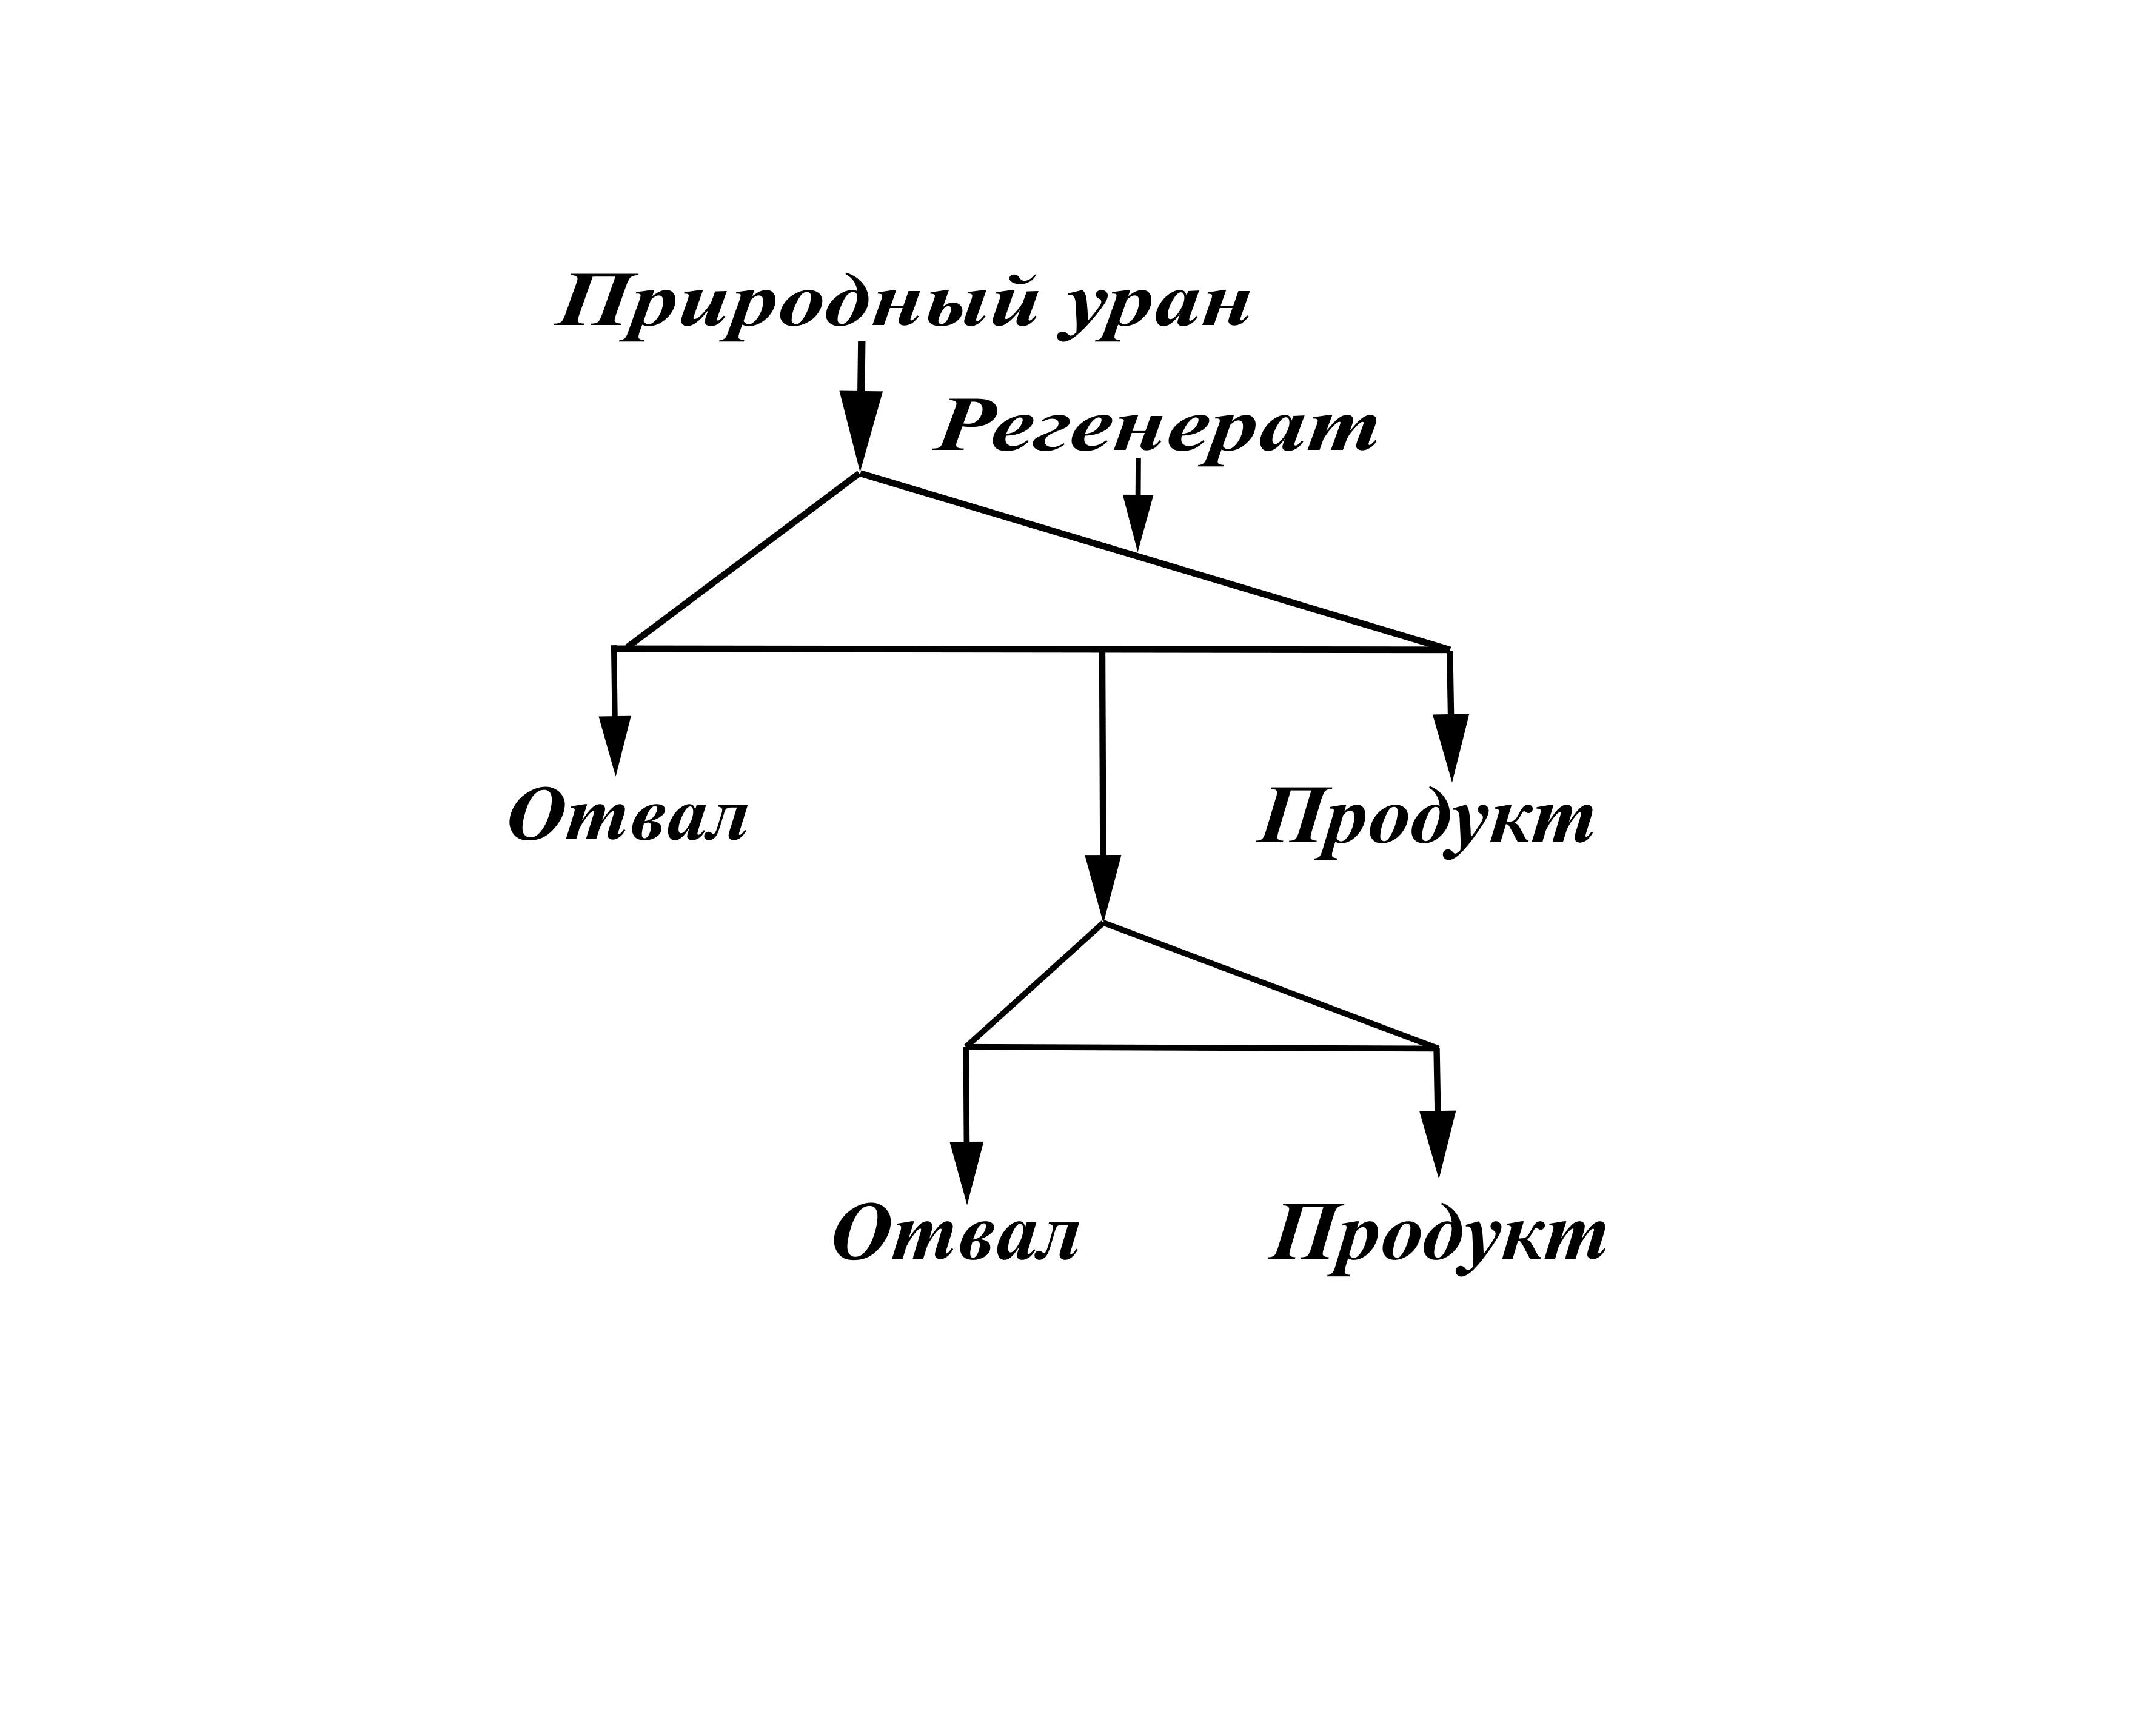
\includegraphics[scale=0.1]{cascades/int_double}}
  \caption{Двойной каскад на основе каскада, получающего очищенный регенерат}\label{fig:int_double}
\end{figure}

Каскады с дополнительным продуктом также могут быть настроены для решения задачи производства разбавителя для ВОУ \cite{palkinPOLUChENIERAZBAVITELYaDLYa2017}, как в \cite{shopenSposobPolucheniyaRazbavitelya2008}. Это дает возможность задействовать наиболее ценный ресурс -- делящийся изотоп $^{235}$U, который преобладает в оружейном уране (> 90\%). Следует отметить, что природный уран, содержание $^{235}$U в котором намного меньше, чем в ВОУ, обычно не очень подходит в качестве разбавителя для ВОУ из-за присутствия в нем $^{234}$U -- сильного альфа-излучателя. Поэтому в качестве разбавителя необходимо использовать изотопную композицию с пониженным содержанием $^{234}$U, поэтому обычно используется обогащенный отвальный уран. Так, в ходе реализации сделки ВОУ-НОУ \cite{korotkevichRealizaciyaProgrammyVOUNOU2003}, использовали наработанный из отвалов разделительного производства обогащенный до 1,5\% разбавитель (патент 2479489) \cite{SposobPolucheniyaRazbavitelya}.


На рис. \ref{fig:double_palk} первый каскад, питаемый регенератом, извлекает изотопы $^{232}$U, $^{234}$U на легком конце, а второй каскад дополнительно подпитывается природным ураном. Такая модификация, как показал Палкин, позволяет «глубоко очищать» обработанную смесь от $^{232}$U, $^{234}$U и уменьшать  $^{236}$U, оставаясь в рамках требуемых ограничений. Этого можно достичь с помощью каскадной оптимизации концентрации $^{232}$U в продукте, варьируя точку подачи, минимизируя количество газовых центрифуг, и $^{235}$U, свободный от вредного $^{232}$U, будет получен на более тяжелом конце каскада. Этот этап предлагается сделать для подготовки лучшей композиции для последующих этапов обогащения. \textcolor{red}{Потерял первоисточник}
\begin{figure}[ht]
  \centerfloat{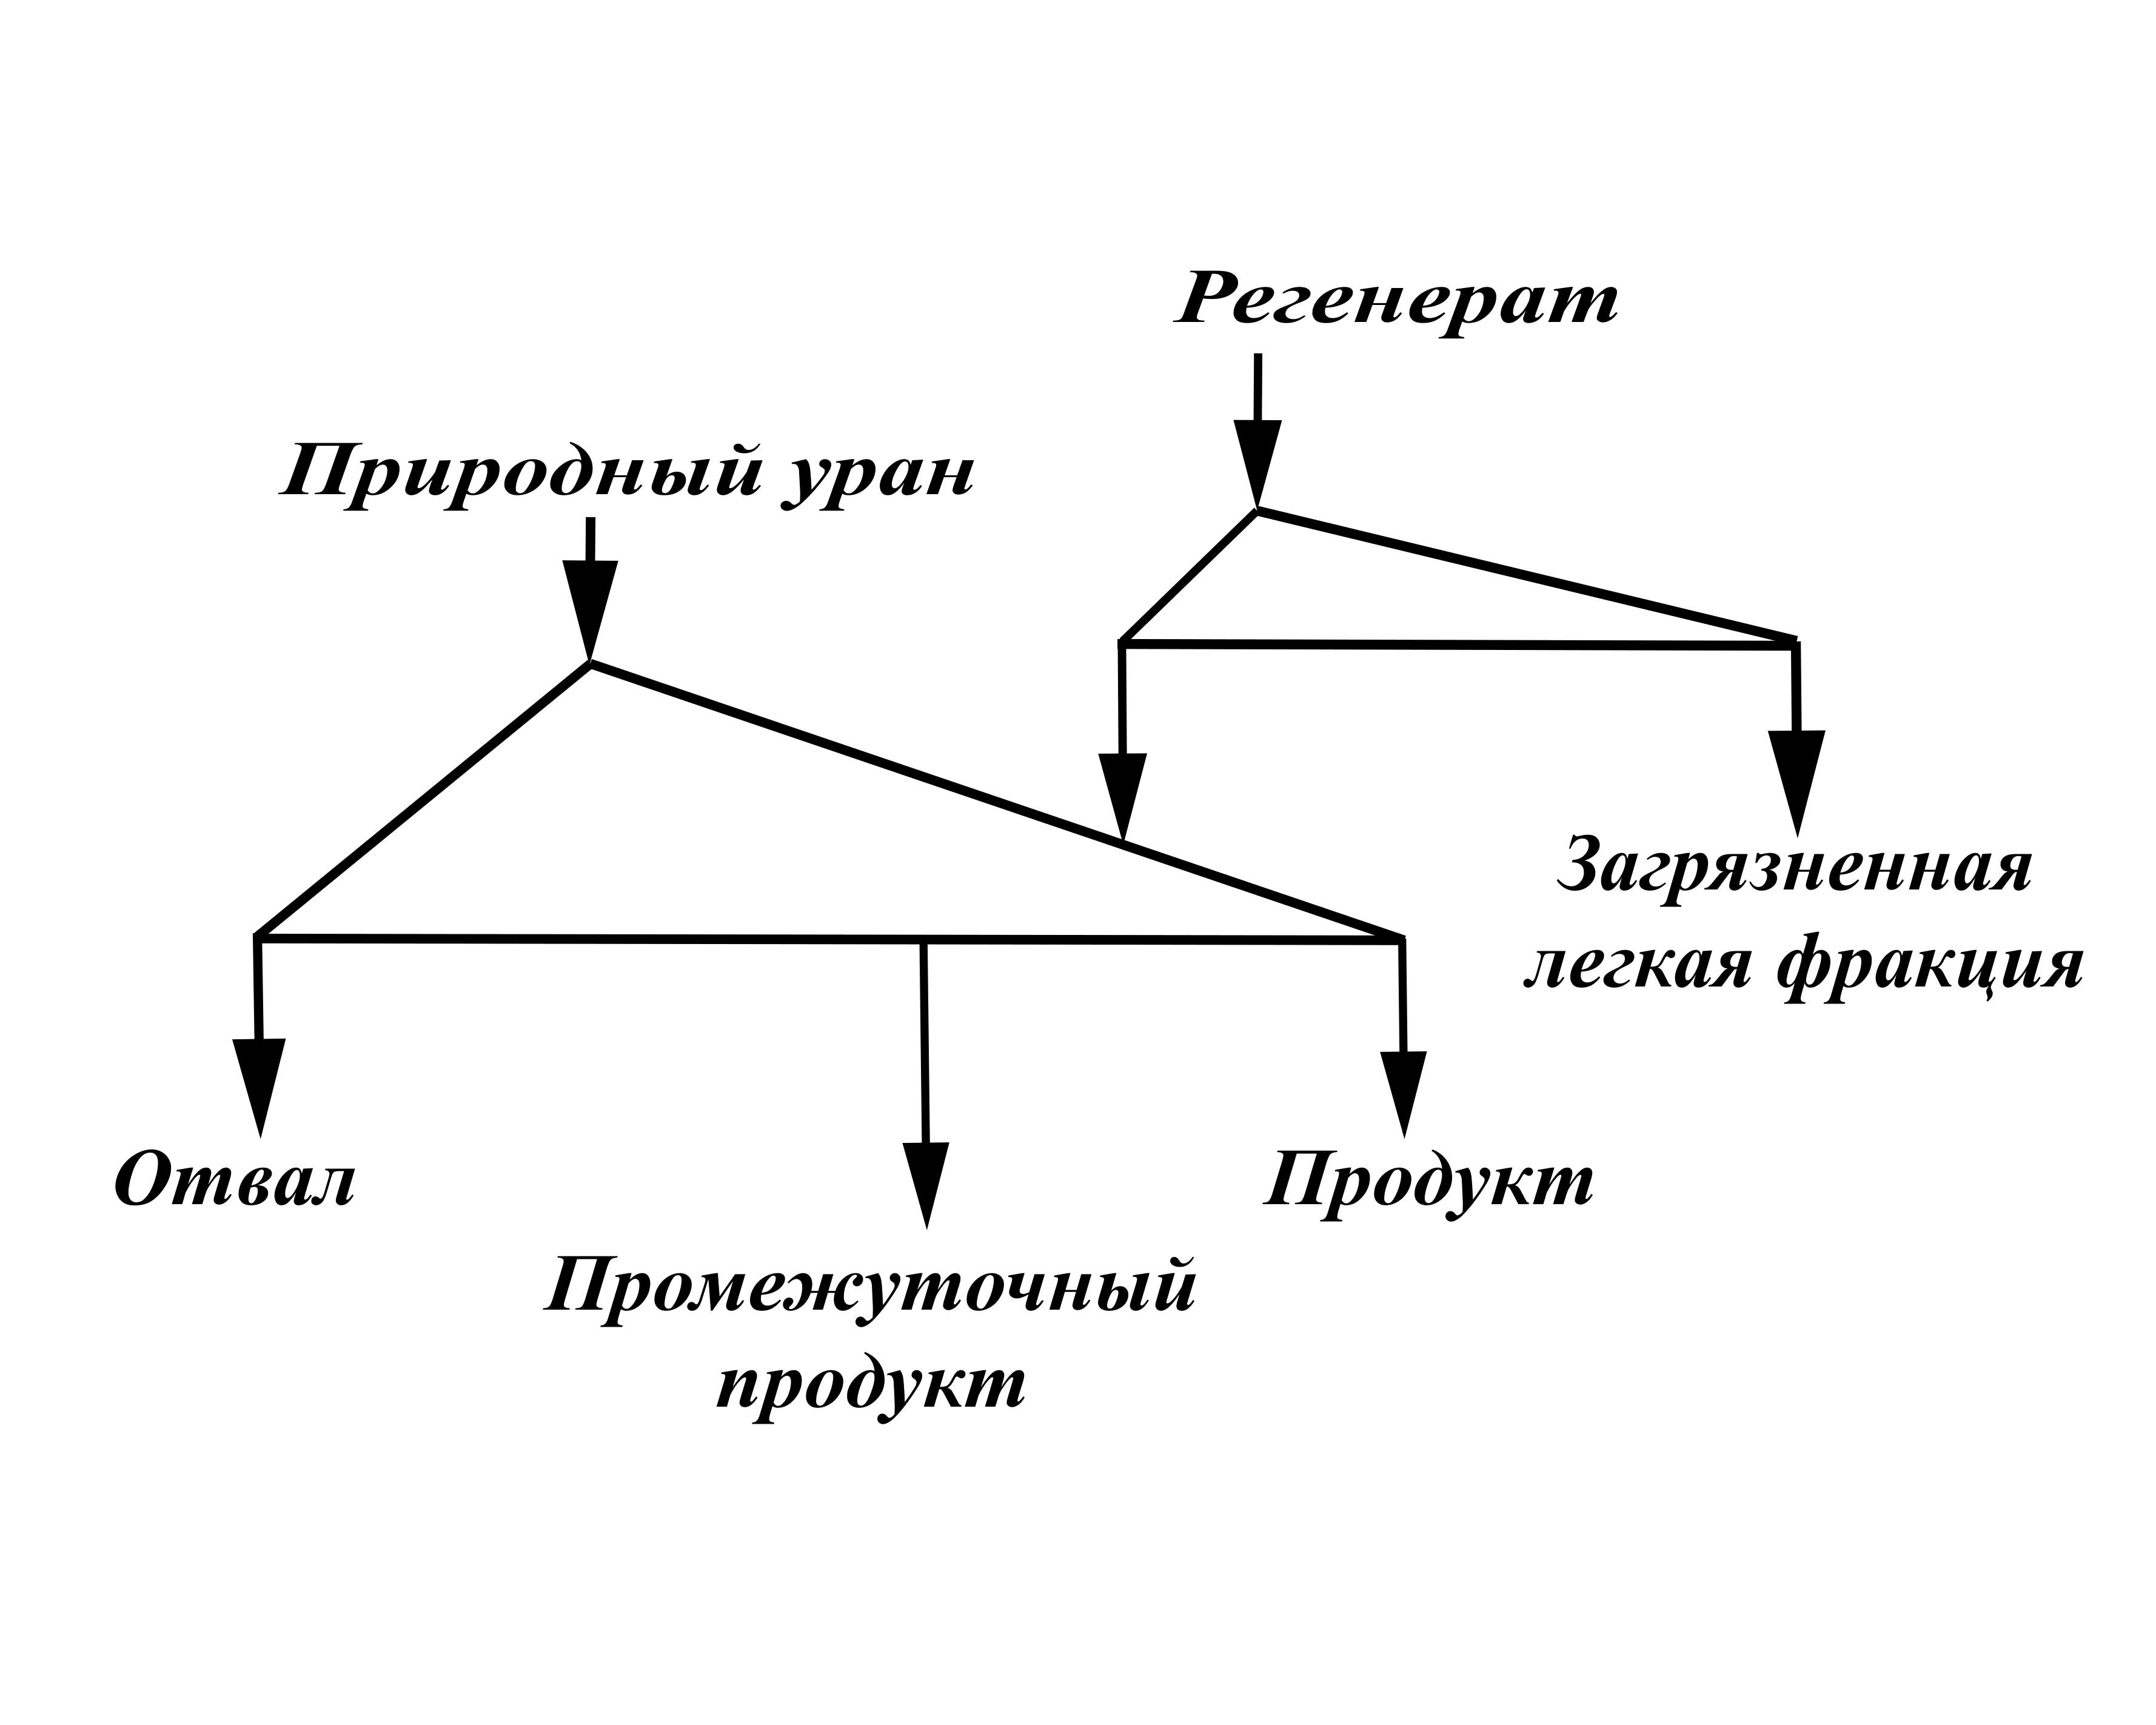
\includegraphics[scale=0.1]{cascades/double_palk}}
  \caption{Двойной каскад, использующий две стадии очистки}\label{fig:double_palk}
\end{figure}

Продолжая примеры схем, в патенте 2497210 \cite{SposobIzotopnogoVosstanovleniyac} приводится способ производства изотопно-восстановленного регенерированного урана, отбирая его из разделительной ступени газовых центрифуг центральной части второго каскада (рис. \ref{fig:double_crazy}).
\begin{figure}[ht]
  \centerfloat{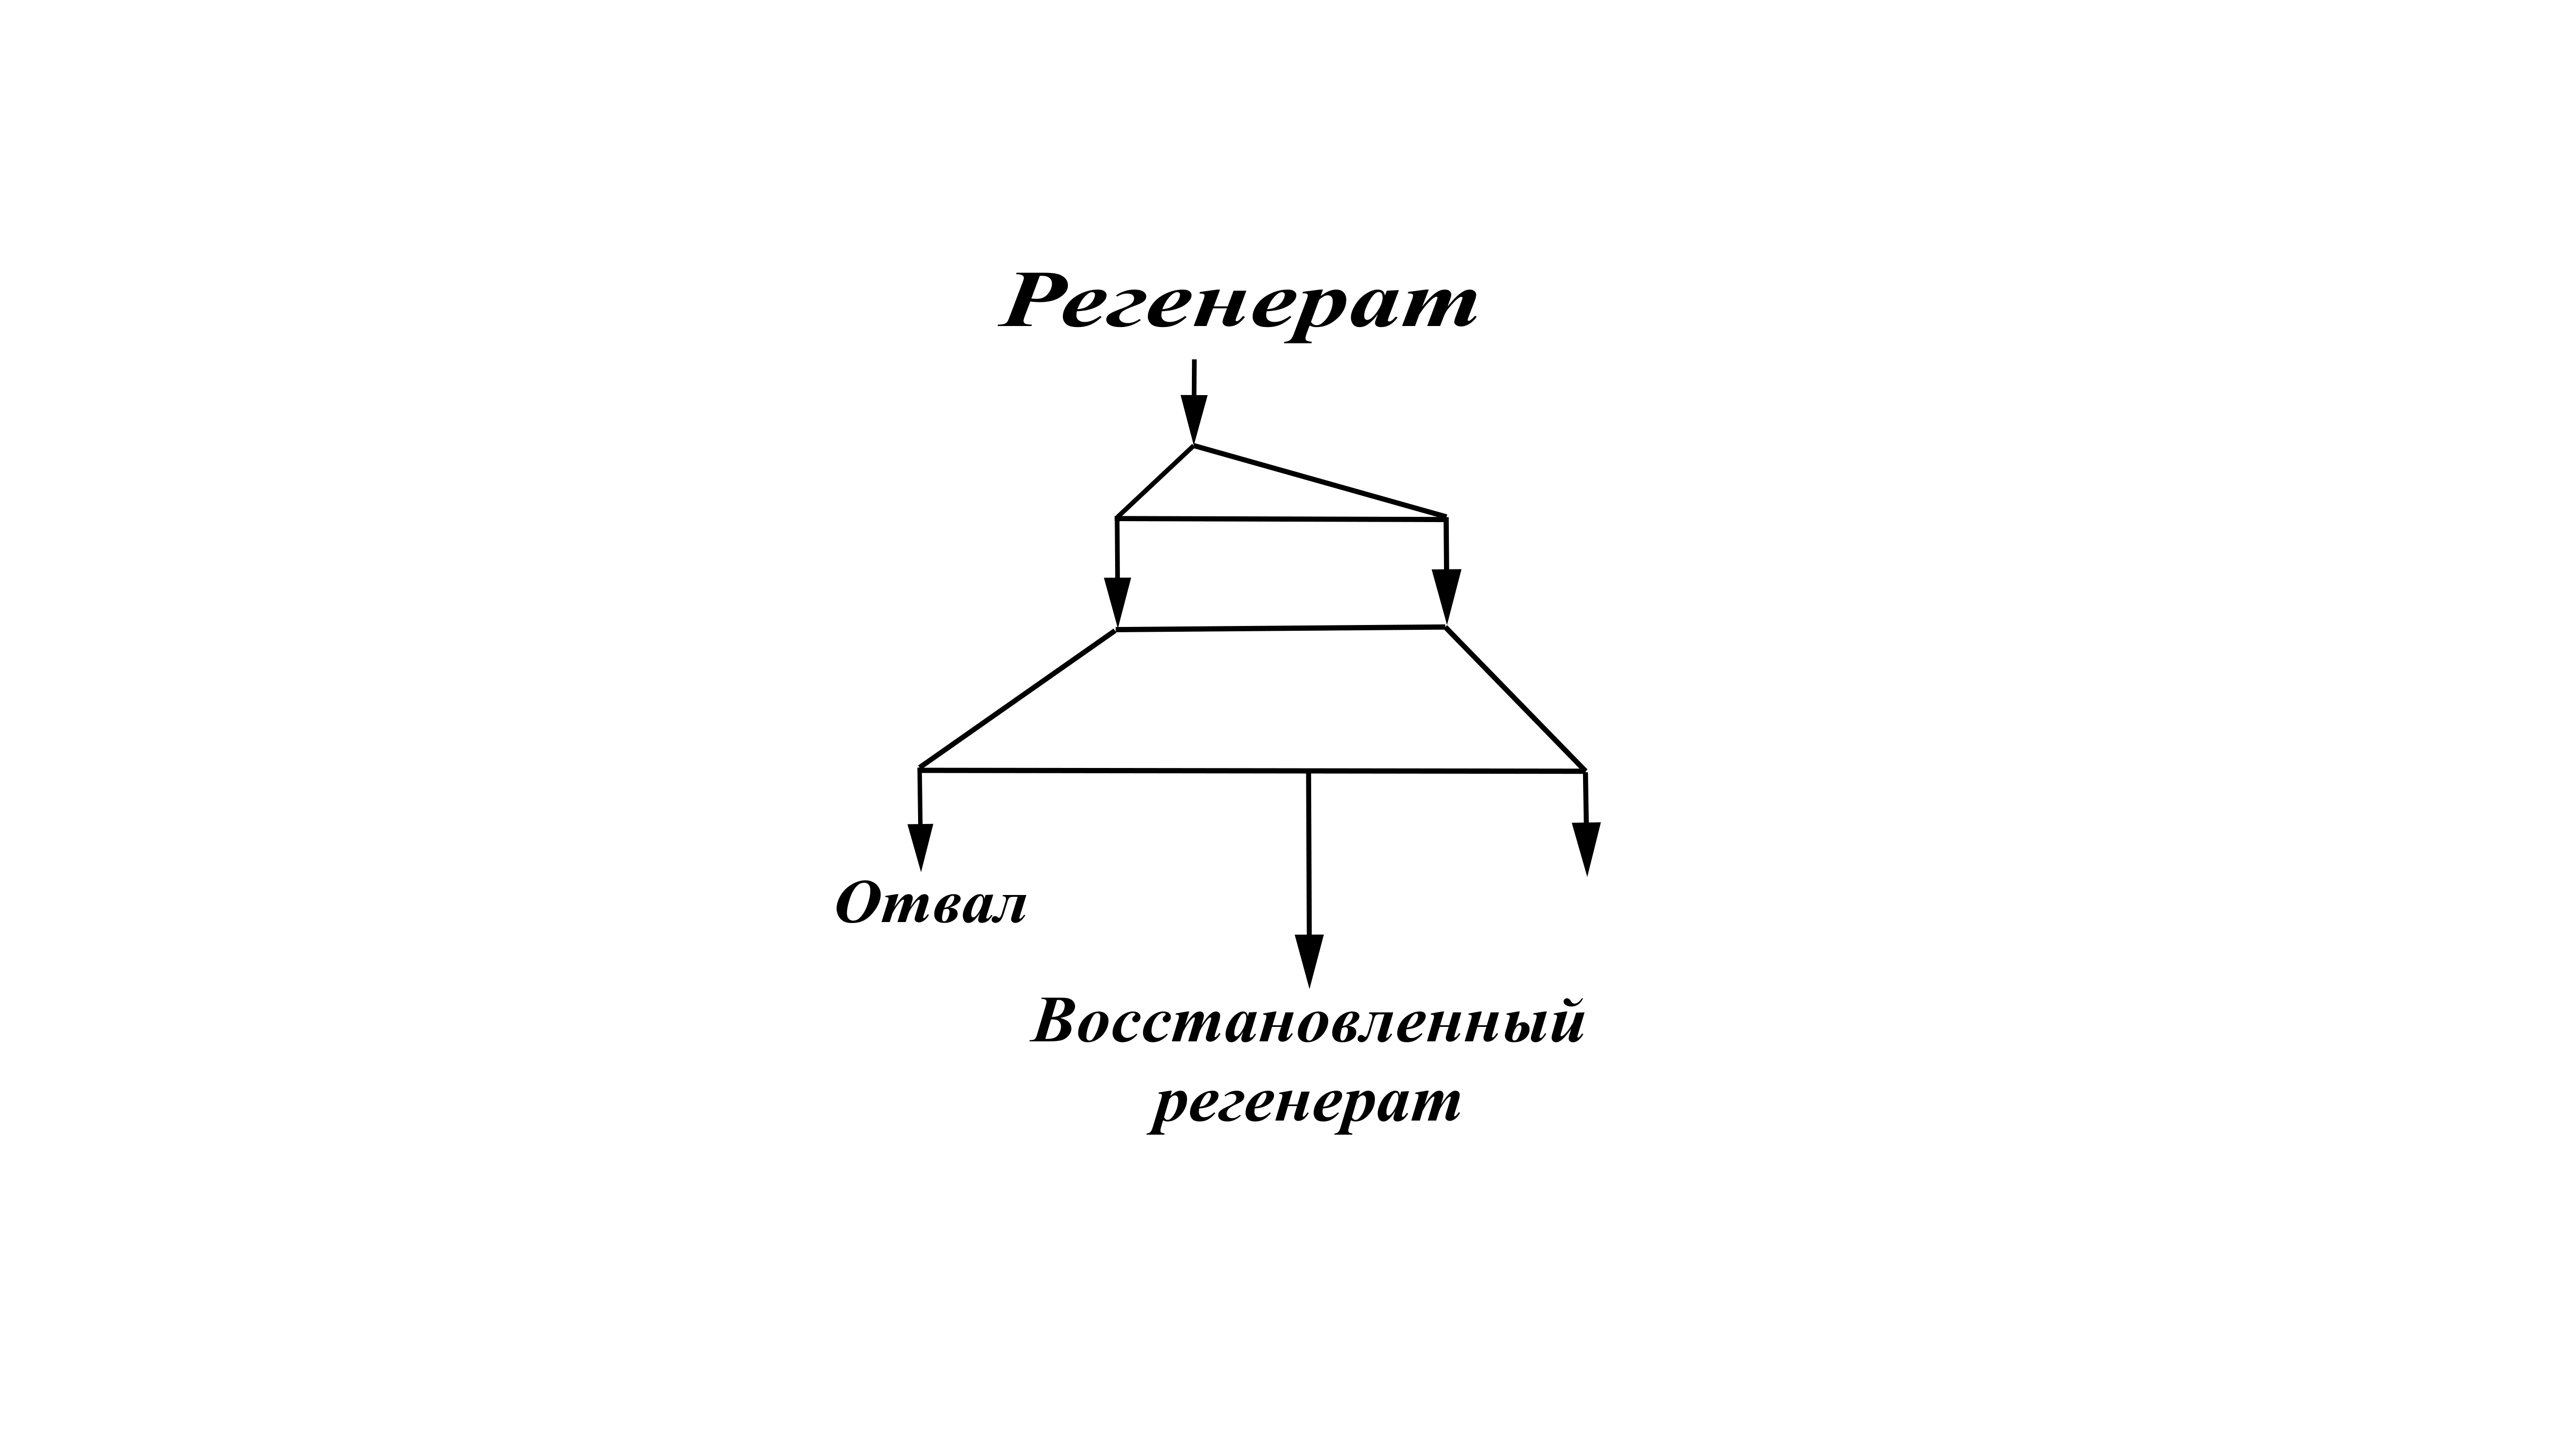
\includegraphics[scale=0.1]{cascades/double_crazy}}
  \caption{Двойной каскад, производящий восстановленный регенерат в промежуточном потоке отбора}\label{fig:double_crazy}
\end{figure}

Зная все эти схемы и их принципы работы, можно легко создать конфигурацию любой сложности, которая будет наиболее подходящей для задачи производства НОУ, с которой прийдется столкнуться.Например, способ построения каскадов, могут представлять собой следующую конфигурацию (рис. \ref{double_3feeds}), которая была представлена в \cite{smirnovDilutionRecycledUranium2015} и получила дальнейшее развитие в \cite{smirnovEvaluatingEffectivenessDilution2016}.
\begin{figure}[ht]
  \centerfloat{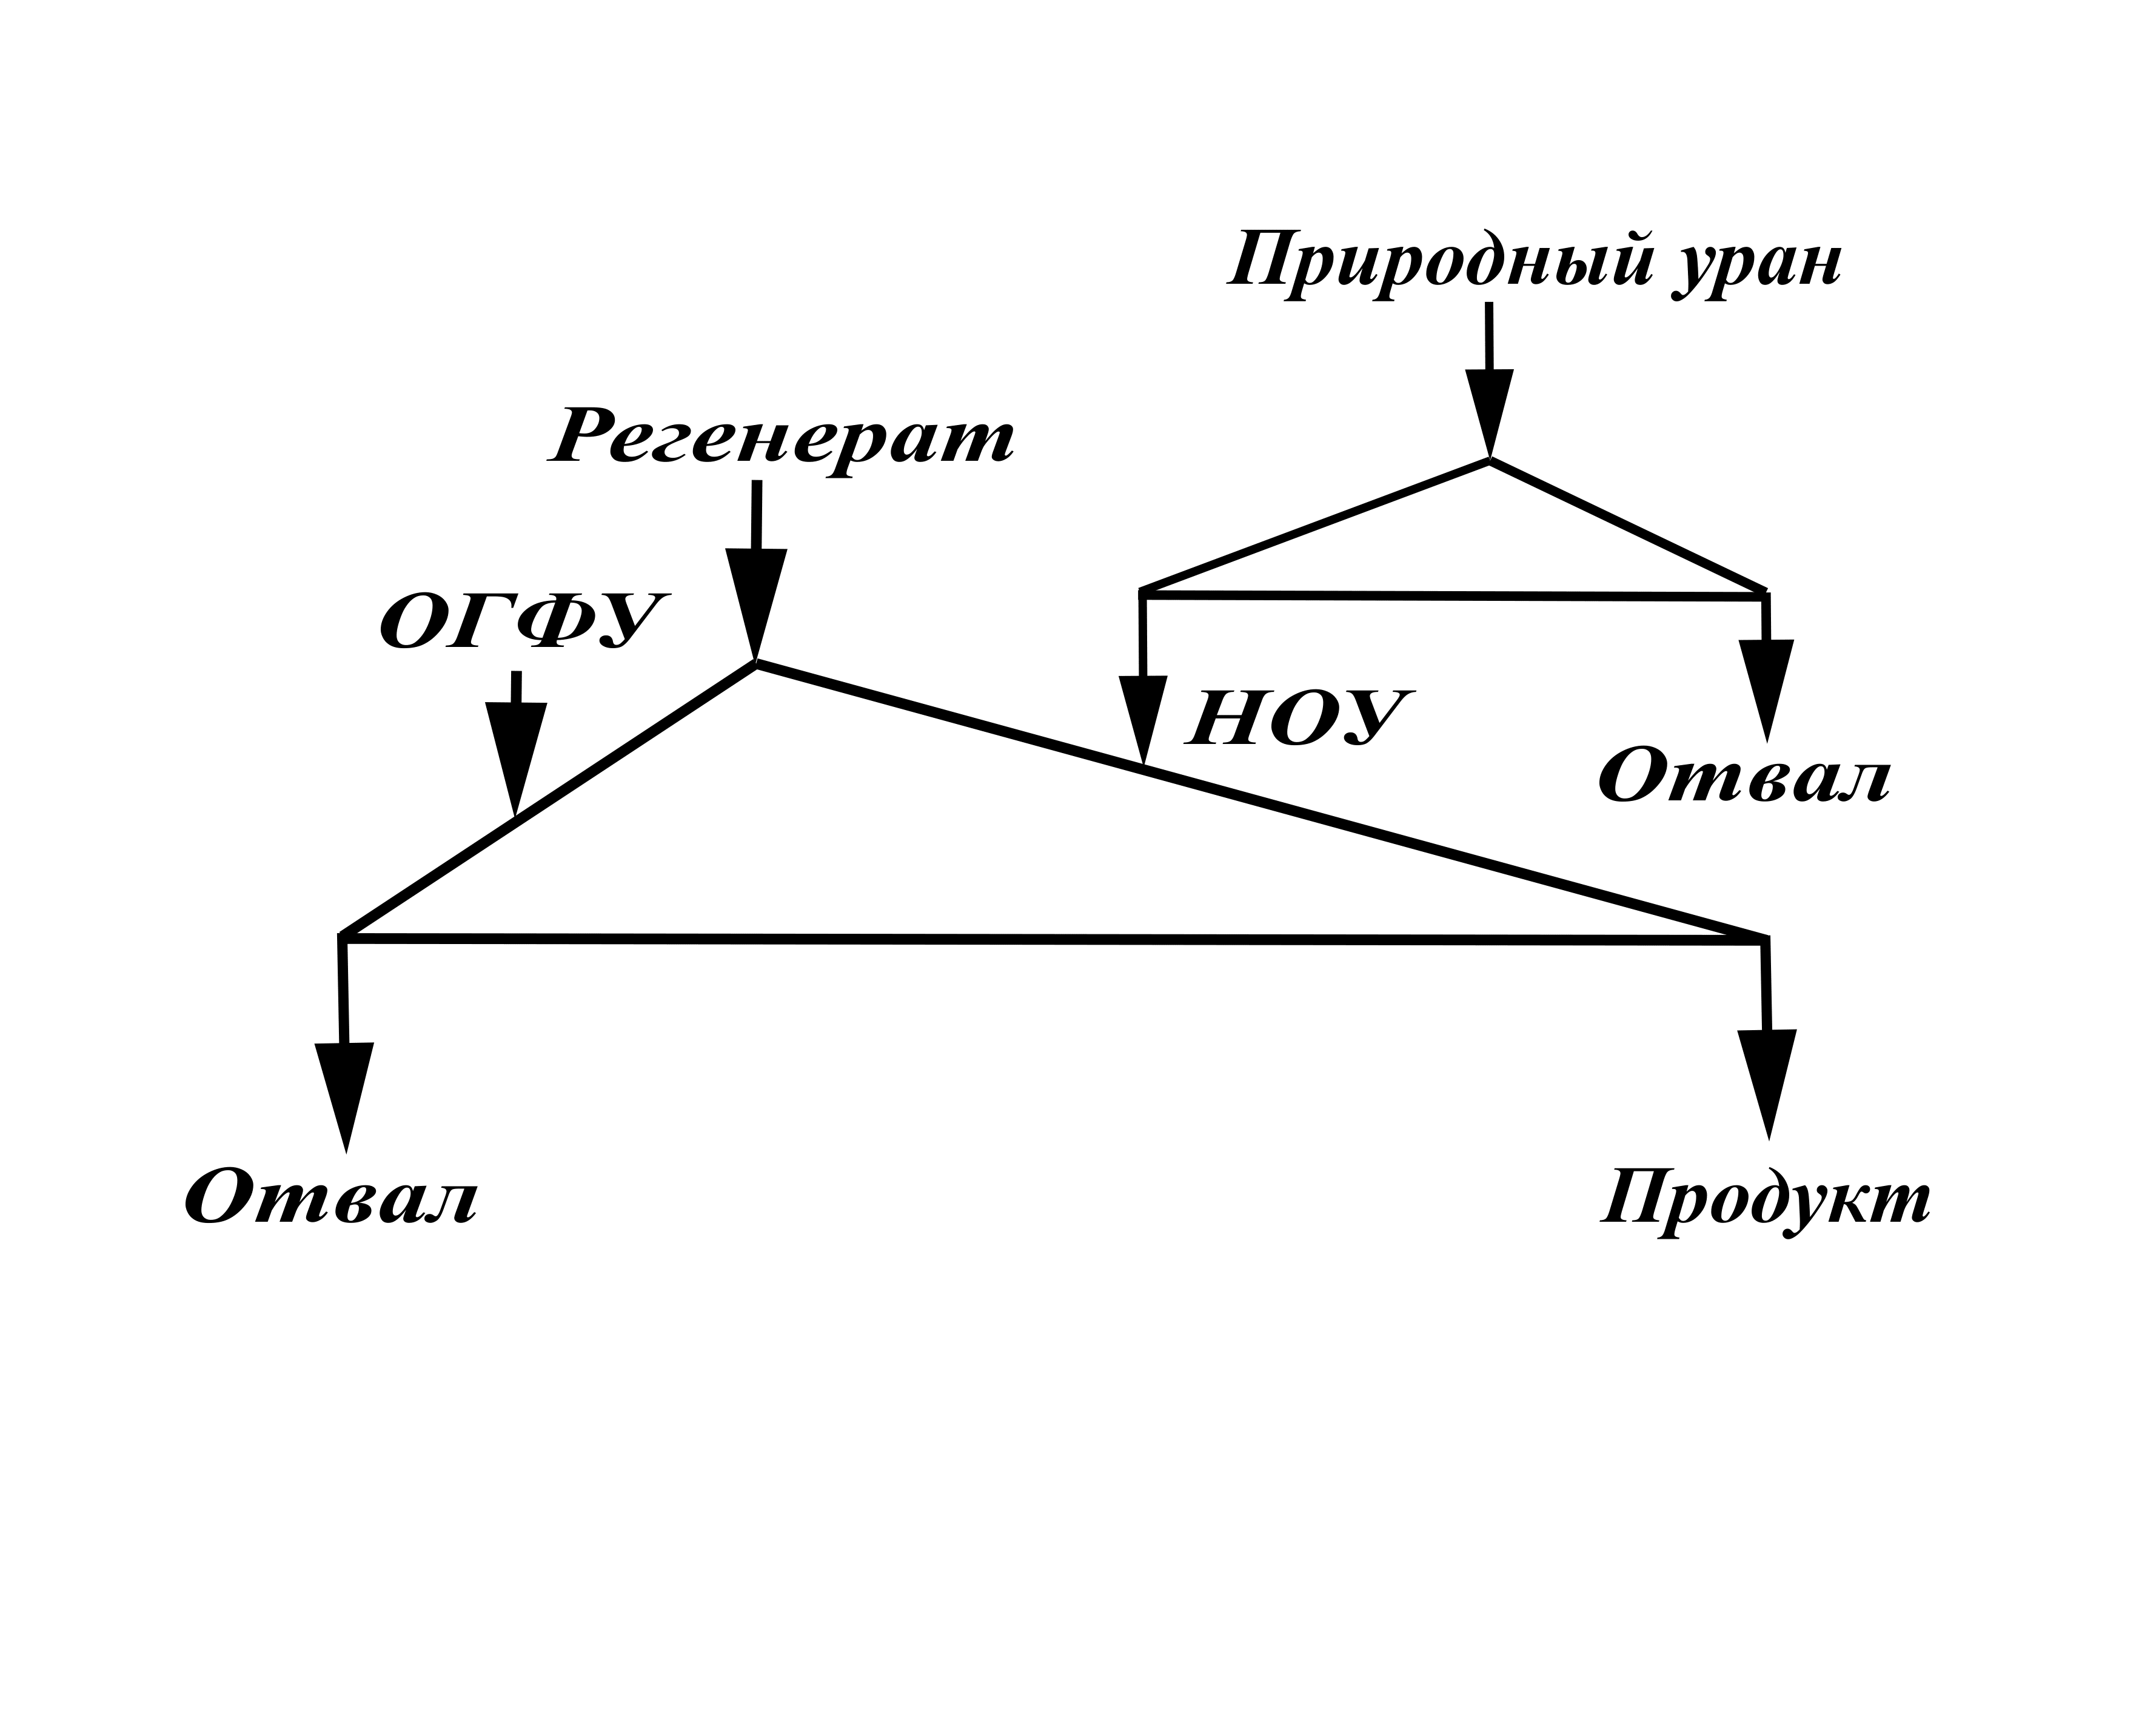
\includegraphics[scale=0.1]{cascades/double_3feeds}}
  \caption{Двойной каскад, использующий каскад с тремя питаниями}\label{fig:double_3feeds}
\end{figure}

Такие схемы как изображенные на рис. \ref{fig:double_3feeds, fig:triple}) можут быть идеальным решением для некоторого класса задач, предоставляя уникальную гибкость в подстройке желаемых кровней экономии природного урана, работы разделения, или же задействования ОГФУ. Подобные структуры могут быть созданы различными способами из всего набора вышеупомянутых схем. Так, в \ref{sec:ch2/sec5.2} будет предложен вариант компоновки наиболее продвинутой на сегодняшний день схемы.


Приведенный критический анализ различных каскадных схем позволяет нам ближе рассмотреть возможные области применения и, таким образом, позволяет более осознанно выбирать конфигурацию для каждой обособленной практической задачи. То есть не представляется возможным остановиться на единственном универсально оптимальном варианте, а лишь можно отметить частные положительные стороны. Таким образом, этот обзор может быть использован в качестве основы для дальнейших научных, технических и технико-экономических обоснований крупномасштабного повторного использования ядерных материалов в различных топливных циклах. Такое исследование и будет проведено далее в данной диссертационной работе.

Завершая обзор предложенных методов повторного обогащения, следует отметить, что до сих пор нет ответа на вопрос, какая из схем по своей природе лучше и эффективнее. Основная причина заключается в том, что из-за принципиальной разницы между предлагаемыми схемами с точки зрения набора параметров, таких как затраты РР, природного урана и произведенных побочных продуктов/отходов, при оценке эффективности рассматриваемых схем невозможно использовать единый критерий эффективности. Существуют попытки сконструировать обобщающий критерий \textcolor{red}{Не находится (опубликованная?) работа с Родионовой}. Следовательно, невозможно дать однозначный ответ на вопрос о том, какую из схем применять для конкретного состава регенерата. Если мы в нашем анализе не будем ограничиваться интересами обогатительного производства, то ответ можно искать в технико-экономическом обосновании, которое будет учитывать не только затраты, связанные непосредственно с разделительным производством (такие как потребление природного урана или ЕРР), но также другие компоненты. Например, затраты, связанные с хранением радиоактивных отходов двойного каскада, или выгоды от утилизации обедненного урана в каскаде с тремя источниками питания, преимущества для продолжительности топливной кампании, ориентируясь на многократный рецикл. К тому же, окончательный ответ не может быть дан, потому что преимущества каждого каскада неотделимы от долгосрочной стратегии отрасли и текущих рыночных цен, а между ними прийдется искать компромиссное решение ввиду нацеленности на долгосрочную перспективу построения ЗЯТЦ. Исходя их вышесказанного расчеты каскадов необходимо создавать программные комплексы ка кинструменты поддержки принятия решений, объединяя при этом соседствующие технологические цепочки, чтобы давать более широкую картину. (те, кто занимается реакторными кодами, используют этот подход, объединяя расчет нейтронно-физический с тепло-гидравлическим, называя это "coupling").  Это особенно важно для долгосрочного горизонта планирования, который тем более необходим для стратегии, связанной с замыканием ЯТЦ, а значит, с б`ольшими затратами на начальной стадии, что вытекает в повышенные риски, единственный способ смягчать которые -- повышать качество прогнозного планирования.


\section{Определение направлений дальнейших исследований}

\subsection{Поиск альтернативных конфигураций каскадов}
Дальнейшая работа предполагает на основе вычислительных экспериментов и анализа закономерностей массопереноса определение схем каскадов, которые могут быть использованы для обогащения регенерированного урана в рамках многократного рецикла. Эффективными представляются схемы двух следующих типов.

\subsection{Исследование каскадов, использующих дополнительный отбор}
Схемы, производящие в дополнительном отборе очищенный от минорных четных изотопов полупродукт. Такая композиция с уменьшенным содержанием $^{232,234,236}$U, но со схожим с питающей смесью содержанием $^{235}$U, может быть направлена на вход схемы, подобной \ref{fig:diagram1} (2), позволяя добиваться на выходе требуемого содержания по всем изотопам. Однако, вариации таких схемы, обычно имеют дополнительные потоки питания, как представлено на рисунках \ref{fig:add}

\begin{figure}[ht]
  \begin{minipage}[b][][b]{0.49\linewidth}\centering
    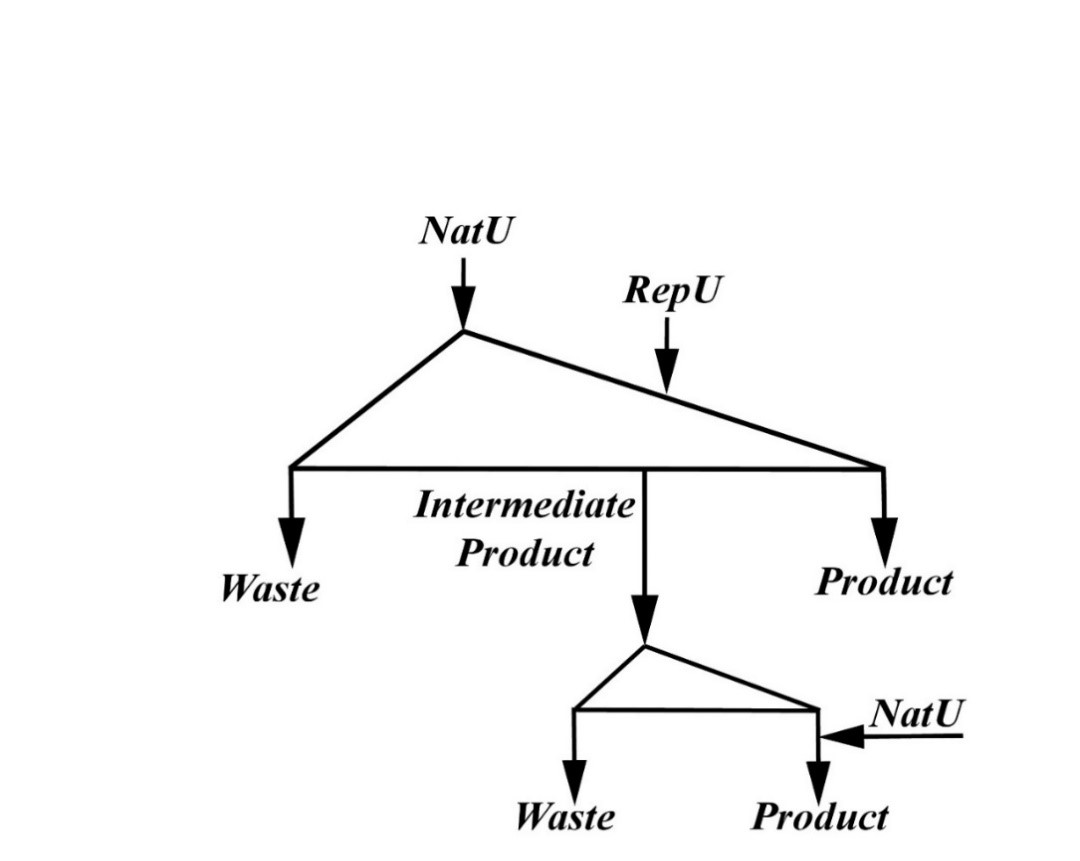
\includegraphics[width=0.9\linewidth]{cascades/add_p} \\ а)
  \end{minipage}
  \hfill
  \begin{minipage}[b][][b]{0.49\linewidth}\centering
    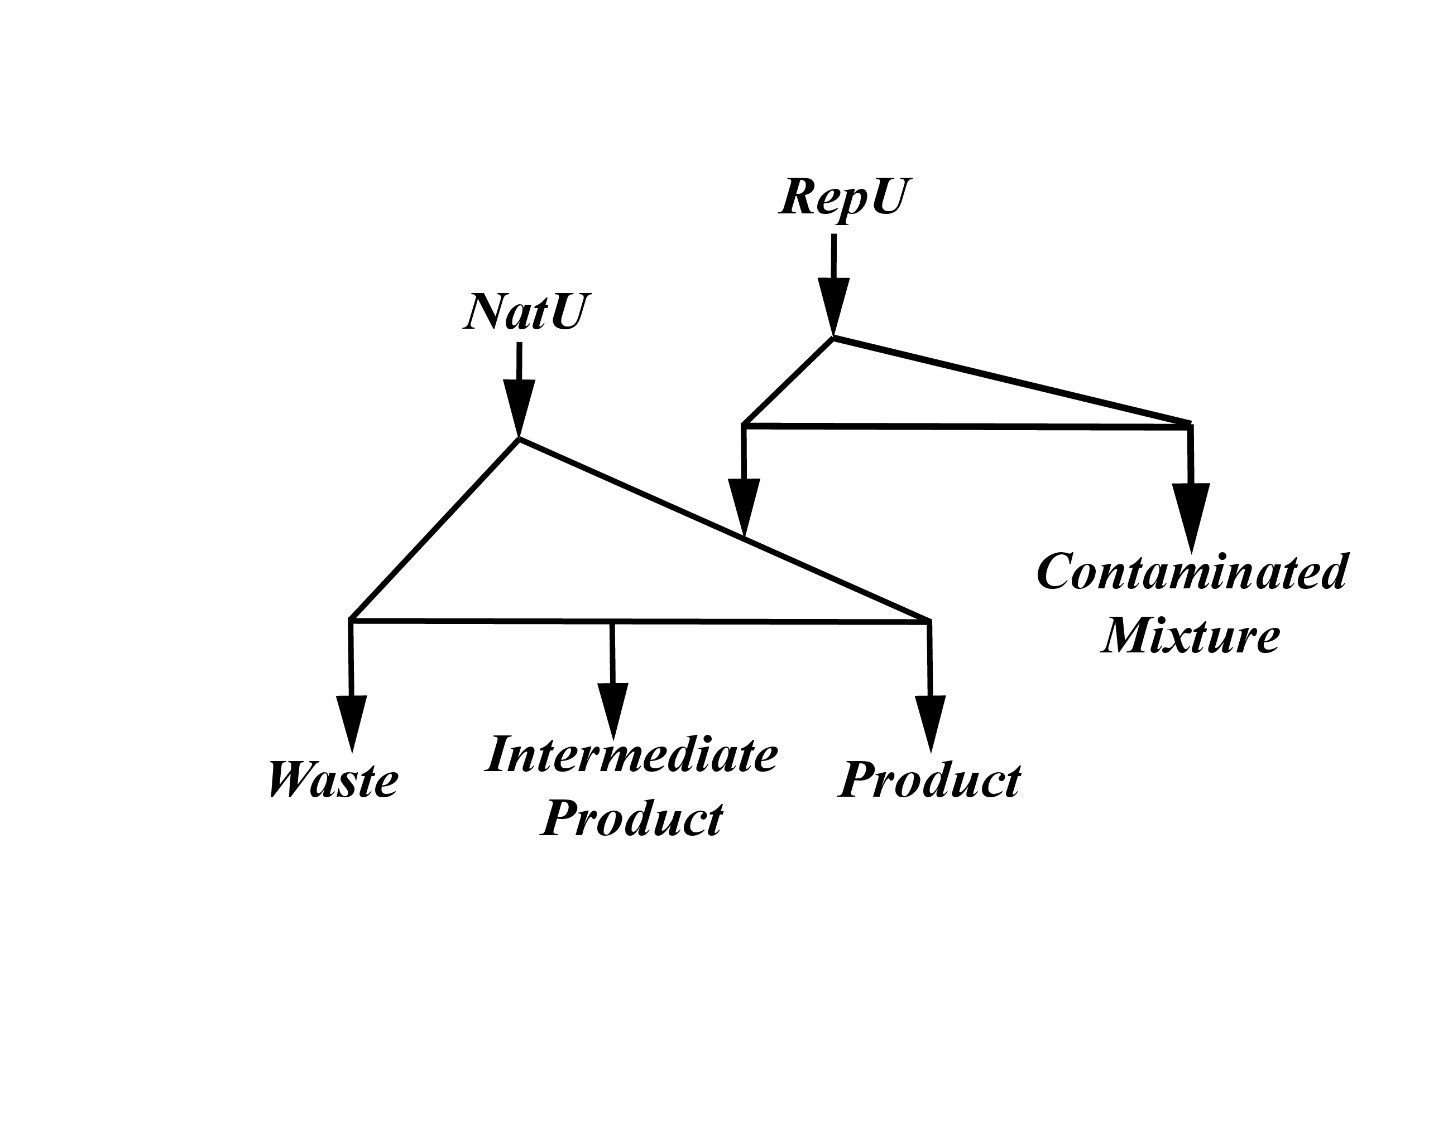
\includegraphics[width=0.9\linewidth]{cascades/add_p2} \\ б)
  \end{minipage}
  \caption{Каскады с дополнительным отбором}
  \label{fig:add}
\end{figure}

Приведенный анализ позволяет заключить, что классификация каскадов по признакам многопоточности и комбинированности (составные схемы) является условной.
Для цели, состоящей в необходимости обогащения регенерата для возврата его в ЯТЦ легководных реакторов в качестве НОУ, выигрышной представляется дихотомия, выделяющая схемы-разбавители и схемы-очистители (от четных изотопов). 

\subsection{Исследование каскадов, использующих смещение точки подачи питания}
С помощью модели квазиидеального каскада необходимо исследование конфигураций, использующих прием в виде варьирования точки подачи питания. Такие схемы тоже требуют анализа на пригодность к приложению в задачах дообогащения регенерированного урана до НОУ, которое может быть использовано в качестве топлива легководных реакторов. Как показано в \cite{palk_2013}, при смещении точки подачи питания каскада относительно оптимума, обеспечивающего минимально возможное число центрифуг, можно существенно изменить концентрацию нецелевых изотопов в отборе и отвале каскада. Такая особенность оптимизации может быть эффективно использована для очистки регенерированного урана от $^{232}$U.

Итак, в данной главе был представлен анализ современных подходов к проблеме повторного обогащения регенерата. Успехи в этой области произошли благодаря достижениям каскадной теории разделения многокомпонентных смесей, произошедшим в последние 60 лет. Следует отметить, что успехи на этом пути подкрепляются усовершенствованием технологии ГЦ, концентрироваться на сегодня является лидирующей в промышленном производстве обогащенного урана.

Оставляя в стороне вопросы, связанные с химической переработкой для получения восстановленной урановой изотопной смеси, предлагается рассмотрение усовершенствованных конфигураций каскадов газовых центрифуг для повторного обогащения этой смеси. 

В расчетных задачах ограничимся следующими предположениями:

 \begin{enumerate}
  \item регенерированный ураном, получен из ОЯТ легководного энергетического реактора. В качестве примера будем рассматривать изотопный состав регенерата из реактора российского дизайна -- ВВЭР.
  \item коэффициент разделения характерен центрифуге российского дизайна.
\end{enumerate}